%File: anonymous-submission-latex-2026.tex
\documentclass[letterpaper]{article} % DO NOT CHANGE THIS
\usepackage[]{aaai2026}  % DO NOT CHANGE THIS
\usepackage[T1]{fontenc}
\usepackage{times}  % DO NOT CHANGE THIS
\usepackage{helvet}  % DO NOT CHANGE THIS
\usepackage{courier}  % DO NOT CHANGE THIS
\usepackage[hyphens]{url}  % DO NOT CHANGE THIS
\usepackage{graphicx} % DO NOT CHANGE THIS
\urlstyle{rm} % DO NOT CHANGE THIS
\def\UrlFont{\rm}  % DO NOT CHANGE THIS
\usepackage{natbib}  % DO NOT CHANGE THIS AND DO NOT ADD ANY OPTIONS TO IT
\usepackage{caption} % DO NOT CHANGE THIS AND DO NOT ADD ANY OPTIONS TO IT
\frenchspacing  % DO NOT CHANGE THIS
\setlength{\pdfpagewidth}{8.5in} % DO NOT CHANGE THIS
\setlength{\pdfpageheight}{11in} % DO NOT CHANGE THIS
%
% These are recommended to typeset algorithms but not required. See the subsubsection on algorithms. Remove them if you don't have algorithms in your paper.
\usepackage{algorithm}
\usepackage{algorithmic}

\usepackage{amsmath} 
\usepackage{amssymb}  % 为了使用 \checkmark
\usepackage{pifont}   % 为了使用 \ding{55}

\usepackage{multirow}
\usepackage[table,xcdraw]{xcolor}

\usepackage{booktabs}
\usepackage{longtable}
\usepackage{caption}
\usepackage{makecell} 
\usepackage{hyperref}

%
% These are are recommended to typeset listings but not required. See the subsubsection on listing. Remove this block if you don't have listings in your paper.
\usepackage{newfloat}
\usepackage{listings}

\usepackage{xcolor}  % 颜色包
\usepackage{todonotes}

% \usepackage{abstract}
% \renewcommand{\abstractnamefont}{\normalfont\bfseries}
% \renewcommand{\abstracttextfont}{\normalfont\normalsize}
\newenvironment{AAAIFrontBlock}
  {\twocolumn[\begin{@twocolumnfalse}]}
  {\end{@twocolumnfalse}]}

\newcommand{\hongzhang}[1]{\textcolor{red}{[Hongzhang: #1]}}
%\newcommand{\todo}[2]{\textcolor{red}{#1}}           % TODO comments
% \newcommand{\zhtang}[1]{[\textcolor{purple}{ZHTang: #1}]}
% \usepackage{ulem}
% \newcommand{\du}[1]{{\color{blue}{\bf du:} #1}}

\DeclareCaptionStyle{ruled}{labelfont=normalfont,labelsep=colon,strut=off} % DO NOT CHANGE THIS
\lstset{%
	basicstyle={\footnotesize\ttfamily},% footnotesize acceptable for monospace
	numbers=left,numberstyle=\footnotesize,xleftmargin=2em,% show line numbers, remove this entire line if you don't want the numbers.
	aboveskip=0pt,belowskip=0pt,%
	showstringspaces=false,tabsize=2,breaklines=true}
\floatstyle{ruled}
\newfloat{listing}{tb}{lst}{}
\floatname{listing}{Listing}
%
% Keep the \pdfinfo as shown here. There's no need
% for you to add the /Title and /Author tags.
\pdfinfo{
/TemplateVersion (2026.1)
}

% DISALLOWED PACKAGES
% \usepackage{authblk} -- This package is specifically forbidden
% \usepackage{balance} -- This package is specifically forbidden
% \usepackage{color (if used in text)
% \usepackage{CJK} -- This package is specifically forbidden
% \usepackage{float} -- This package is specifically forbidden
% \usepackage{flushend} -- This package is specifically forbidden
% \usepackage{fontenc} -- This package is specifically forbidden
% \usepackage{fullpage} -- This package is specifically forbidden
% \usepackage{geometry} -- This package is specifically forbidden
% \usepackage{grffile} -- This package is specifically forbidden
% \usepackage{navigator} -- This package is specifically forbidden
% (or any other package that embeds links such as navigator or hyperref)
% \indentfirst} -- This package is specifically forbidden
% \layout} -- This package is specifically forbidden
% \multicol} -- This package is specifically forbidden
% \nameref} -- This package is specifically forbidden
% \usepackage{savetrees} -- This package is specifically forbidden
% \usepackage{setspace} -- This package is specifically forbidden
% \usepackage{stfloats} -- This package is specifically forbidden
% \usepackage{tabu} -- This package is specifically forbidden
% \usepackage{titlesec} -- This package is specifically forbidden
% \usepackage{tocbibind} -- This package is specifically forbidden
% \usepackage{ulem} -- This package is specifically forbidden
% \usepackage{wrapfig} -- This package is specifically forbidden
% DISALLOWED COMMANDS
% \nocopyright -- Your paper will not be published if you use this command
% \addtolength -- This command may not be used
% \balance -- This command may not be used
% \baselinestretch -- Your paper will not be published if you use this command
% \clearpage -- No page breaks of any kind may be used for the final version of your paper
% \columnsep -- This command may not be used
% \newpage -- No page breaks of any kind may be used for the final version of your paper
% \pagebreak -- No page breaks of any kind may be used for the final version of your paperr
% \pagestyle -- This command may not be used
% \tiny -- This is not an acceptable font size.
% \vspace{- -- No negative value may be used in proximity of a caption, figure, table, section, subsection, subsubsection, or reference
% \vskip{- -- No negative value may be used to alter spacing above or below a caption, figure, table, section, subsection, subsubsection, or reference

\setcounter{secnumdepth}{0} %May be changed to 1 or 2 if section numbers are desired.

% The file aaai2026.sty is the style file for AAAI Press
% proceedings, working notes, and technical reports.
%

% Title

% Your title must be in mixed case, not sentence case.
% That means all verbs (including short verbs like be, is, using,and go),
% nouns, adverbs, adjectives should be capitalized, including both words in hyphenated terms, while
% articles, conjunctions, and prepositions are lower case unless they
% directly follow a colon or long dash
\title{GitTaskBench: A Benchmark for Code Agents Solving Real-World Tasks \\ Through Code Repository Leveraging}
% \author{
%     %Authors
%     % All authors must be in the same font size and format.
%     Written by AAAI Press Staff\textsuperscript{\rm 1}\thanks{With help from the AAAI Publications Committee.}\\
%     AAAI Style Contributions by Pater Patel Schneider,
%     Sunil Issar,\\
%     J. Scott Penberthy,
%     George Ferguson,
%     Hans Guesgen,
%     Francisco Cruz\equalcontrib,
%     Marc Pujol-Gonzalez\equalcontrib
% }
% \affiliations{
%     %Afiliations
%     \textsuperscript{\rm 1}Association for the Advancement of Artificial Intelligence\\
%     % If you have multiple authors and multiple affiliations
%     % use superscripts in text and roman font to identify them.
%     % For example,

%     % Sunil Issar\textsuperscript{\rm 2},
%     % J. Scott Penberthy\textsuperscript{\rm 3},
%     % George Ferguson\textsuperscript{\rm 4},
%     % Hans Guesgen\textsuperscript{\rm 5}
%     % Note that the comma should be placed after the superscript

%     1101 Pennsylvania Ave, NW Suite 300\\
%     Washington, DC 20004 USA\\
%     % email address must be in roman text type, not monospace or sans serif
%     proceedings-questions@aaai.org
% %
% % See more examples next
% }

\vspace{10pt}
\author{
\normalsize
\\[0.3em]
    \textbf{\textit{Ziyi Ni}\textsuperscript{1,2 *}}\quad
    \textbf{\textit{Huacan Wang}\textsuperscript{1,* ‡}}\quad
    \textbf{\textit{Shuo Zhang}\textsuperscript{3 *}}\quad
    \textbf{Shuo Lu\textsuperscript{1,2}}\quad
    \textbf{Ziyang He\textsuperscript{4}}\quad
    \textbf{Wang You\textsuperscript{5}}
\\[0.3em]
    \textbf{Zhenheng Tang\textsuperscript{6}}\quad
    \textbf{Yuntao Du\textsuperscript{7}}\quad
    \textbf{Bill Sun\textsuperscript{8}}\quad
    \textbf{Hongzhang Liu\textsuperscript{9,10}}\quad
    \textbf{Sen Hu\textsuperscript{10}}\quad
    \textbf{Ronghao Chen\textsuperscript{10}}
\\[0.3em]
    \textbf{Bo Li\textsuperscript{6}}\quad
    \textbf{Xin Li\textsuperscript{11}}\quad
    \textbf{Chen Hu\textsuperscript{5,‡}}\quad
    \textbf{Binxing Jiao\textsuperscript{5}}\quad
    \textbf{Daxin Jiang\textsuperscript{5,‡}}\quad
    \textbf{Pin Lyu\textsuperscript{2,‡}}
\\[1em]
 \textsuperscript{1}UCAS\quad \textsuperscript{2}CASIA\quad \textsuperscript{3}BUPT\quad \textsuperscript{4}NUS\quad \textsuperscript{5}StepFun\quad
 \textsuperscript{6}HKUST\quad
 \textsuperscript{7}SDU\quad
 \textsuperscript{8}PINAI\quad
 \textsuperscript{9}USYD\quad
 \textsuperscript{10}PKU\quad
 \textsuperscript{11}USTC\quad
\\[1em]
\textsuperscript{\textbf{*}} \textbf{These authors contributed equally to this work.}
\\[0.5em]
\textsuperscript{$\dagger$} \textbf{Corresponding authors:}
\href{mailto:wanghuacan17@mails.ucas.ac.cn}{wanghuacan17@mails.ucas.ac.cn},\quad
  \href{mailto:djiang@stepfun.com}  {djiang@stepfun.com},\quad
  \href{mailto:pin.lv@ia.ac.cn}{pin.lv@ia.ac.cn}
% wanghuacan17@mails.ucas.ac.cn\quad
% djiang@stepfun.com\quad
% pin.lv@ia.ac.cn
\\[1.2em]
}

% REMOVE THIS: bibentry
% This is only needed to show inline citations in the guidelines document. You should not need it and can safely delete it.
% \usepackage{bibentry}
% END REMOVE bibentry


\renewcommand{\floatpagefraction}{0.2}
\nocopyright

\begin{document}

\setfrontabstractmargins{3.2pc}{3.2pc}
\setfrontabstractboxsep{16pt}                   % 盒子内边距
\setfrontabstracttitleskip{1ex}               % 标题与正文距离
\setfrontabstracttitleformat{\centering\bfseries\color{AAAIFrontAbsBorder}\fontsize{12}{13}\selectfont}

% \begin{abstract}
\frontabstract{
Beyond scratch coding, exploiting large-scale code repositories (e.g., GitHub) for practical tasks is vital in real-world software development, yet current benchmarks rarely evaluate code agents in such authentic, workflow-driven scenarios. 
To bridge this gap, we introduce GitTaskBench, a benchmark designed to systematically assess this capability via 54 realistic tasks across 7 modalities and 7 domains. 
Each task pairs a relevant repository with an automated, human-curated evaluation harness specifying practical success criteria. Beyond measuring execution and task success, we also propose the alpha-value metric to quantify the economic benefit of agent performance, which integrates task success rates, token cost, and average developer salaries. Experiments across three state-of-the-art agent frameworks with multiple advanced LLMs show that leveraging code repositories for complex task solving remains challenging: even the best-performing system, \mbox{OpenHands+Claude 3.7}, solves only 48.15\,\% of tasks (\textit{recent progress has pushed the frontier further, with \mbox{RepoMaster+Claude 3.5} achieving a new record of 62.96\%}). Error analysis attributes over half of failures to seemingly mundane yet critical steps like environment setup and dependency resolution, highlighting the need for more robust workflow management and increased timeout preparedness.
By releasing GitTaskBench, we aim to drive progress and attention toward repository-aware code reasoning, execution, and deployment---moving agents closer to solving complex, end-to-end real-world tasks.
\\[0.8em]
\textbf{Benchmark and code:} \url{https://github.com/QuantaAlpha/GitTaskBench}.
\\[0.3em]
\textbf{Our project page: }\url{https://gittaskbench.github.io/}.
% \end{abstract}
}


\frontteaser{
 \vspace{1.2em}
 % \begin{firstpagefigure}
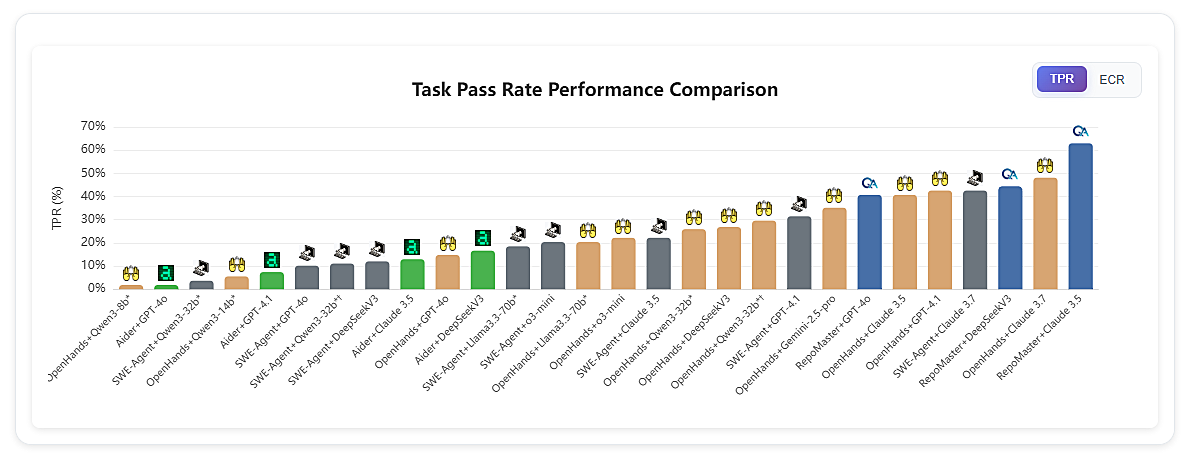
\includegraphics[width=\textwidth]{images/leaderboard.png}
    \captionof{figure}{Up-to-Date Leaderboard: AI agent performance on GitTaskBench evaluation tasks.}
  % \end{firstpagefigure}
}


\maketitle


% % \vspace{4pt}
% \begin{figure*}[!bt]
% \centering 
% 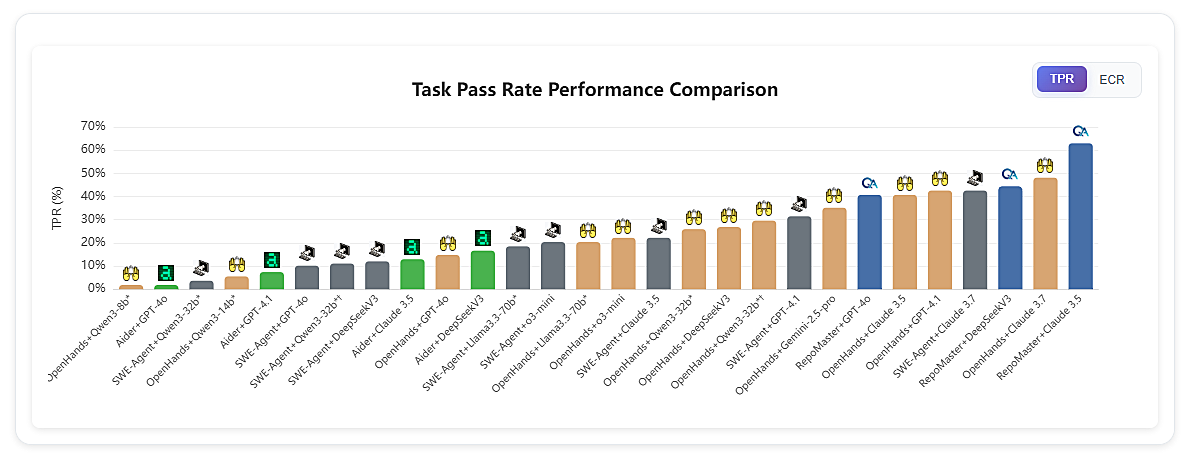
\includegraphics[width=1\textwidth]{images/leaderboard.png}
% \label{Fig.leaderboard} 
% % \vspace{-8pt}
% \end{figure*}


\begin{figure*}[t]
    \centering
    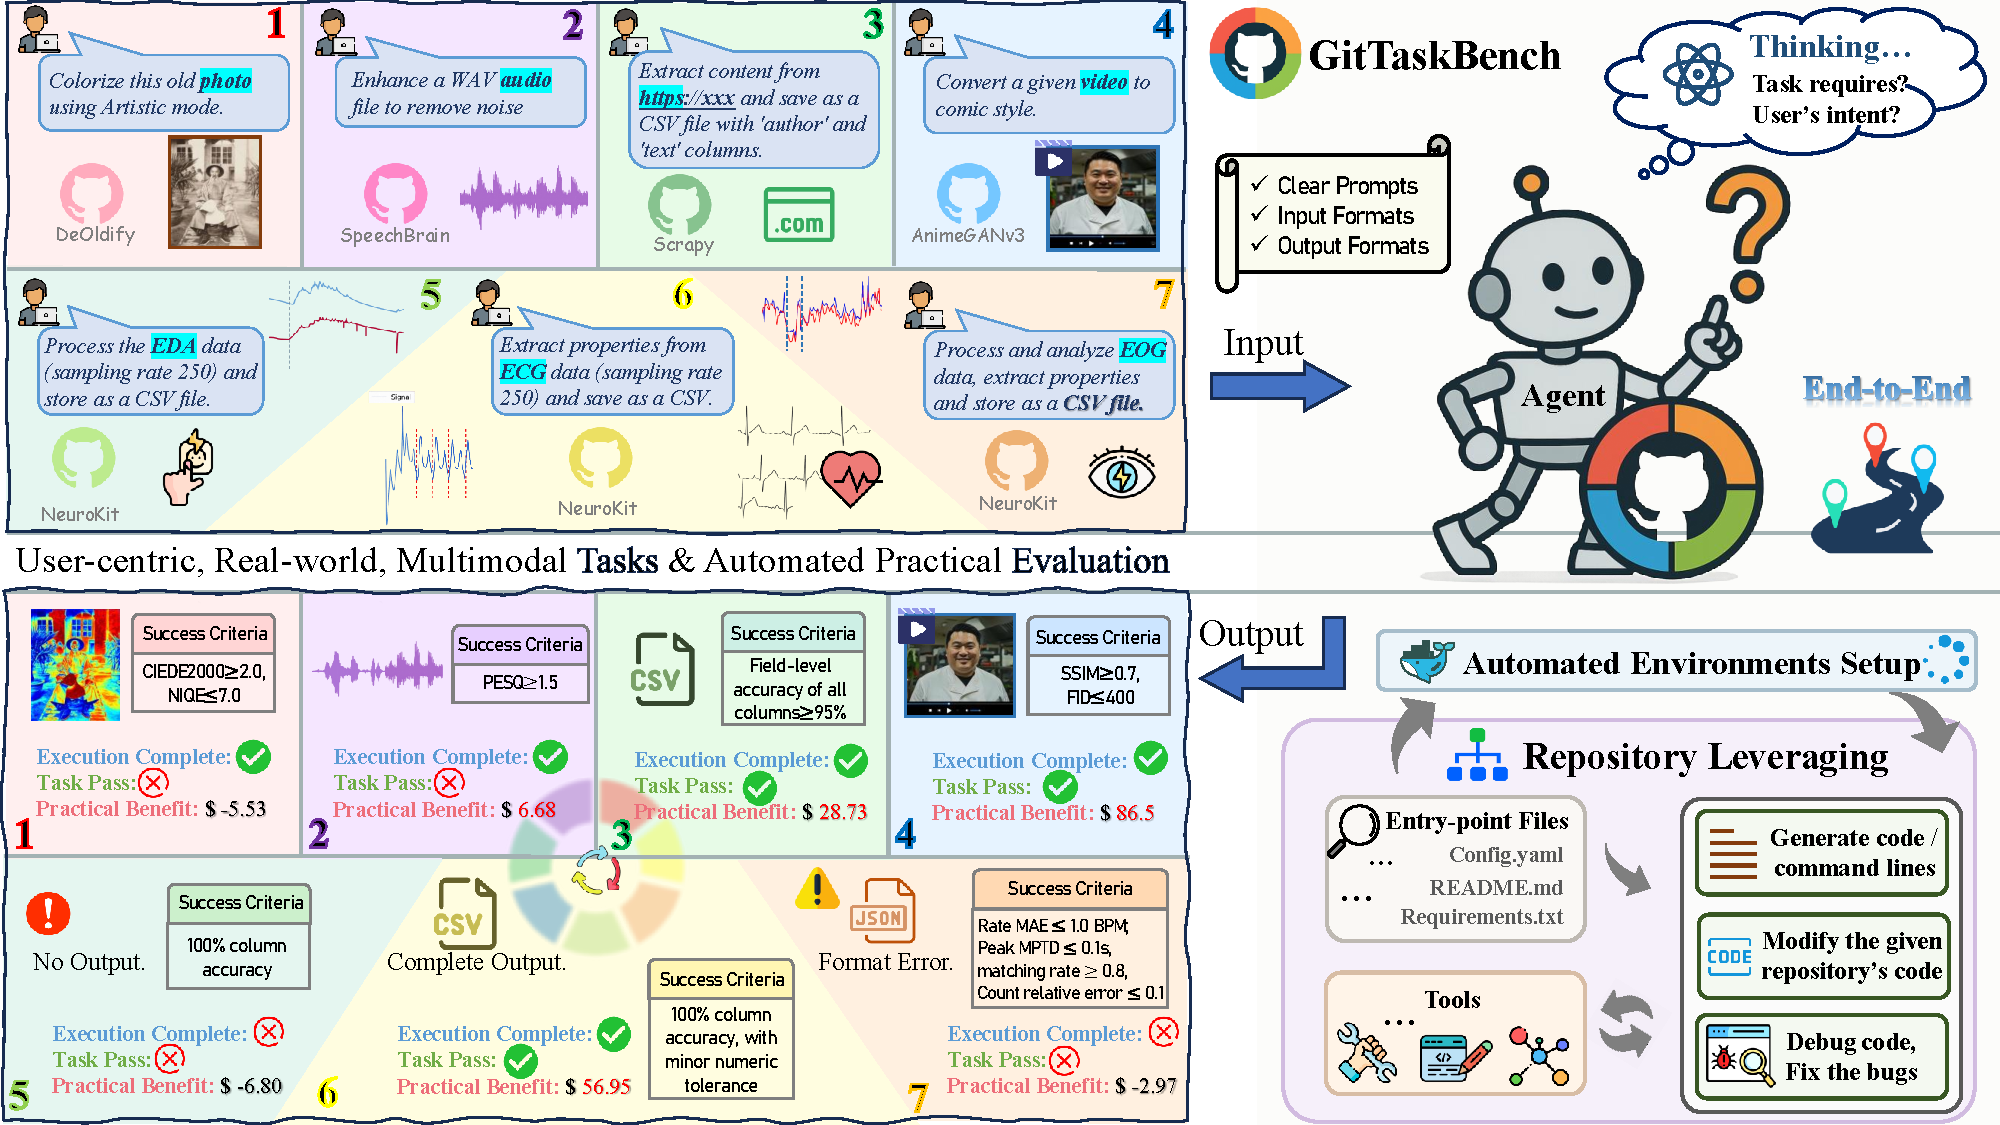
\includegraphics[width=0.975\linewidth]{images/overview_v6.pdf}
    \caption{Overview of GitTaskBench. 7 example real-life tasks from different modalities and their evaluations are shown.}
    \label{fig:overview}
\end{figure*}


\section{Introduction}


In just two years, fueled by the transformative progress of large language model (LLM) agents, an increasing number of code benchmarks have reached saturation~\cite{HumanEval2021,MBPP2021,hendrycks2021measuring,2021codexglue}. 
However, \textbf{most early code-agent works and benchmarks target isolated, static problems}, such as algorithmic tests \cite{hendrycks2021measuring, 2022alphacode, zheng2025livecodebench}, code completion at the function \cite{HumanEval2021, MBPP2021, 2023ds-1000}, class \cite{du2023classeval}, or repository level \cite{liu2023repobench,ding2023crosscodeeval}, or program repair \cite{jimenez2023swe}---\textbf{failing to assess agents’ capacity in real-world problem solving}.

Recent efforts have begun to develop more practical, comprehensive benchmarks.
Some works still focus on code generation, requiring agents to produce increasingly complex code, even generating entire repositories from scratch \cite{yu2024HumanEval-Pro, weirdml, chan2025mle-bench, swe-lancer, paperbench}. 
%
%
However, such a heavy burden remains prohibitively difficult for most current agent systems~\cite{li2024devbench, paperbench}. Moreover, \textbf{focusing solely on code generation overlooks the broader scope of real-world developer practice}~\cite{Adnan2024Manus}, and \textbf{provides diminishing insight into agent capabilities}~\cite{gao2024LLMSurvey}. 
%
Another line of work rethinks evaluation paradigms \cite{2024MAcode-generation} by integrating code generation with external tools or API calls~\cite{API-bank, codeact, ToolEyes, zhuo2024bigcodebench,tang2025the,dong2025can}, thus easing the generation burden but still sidestepping the harder challenge of understanding and repurposing the full repositories. 

However, \textit{real-world programmers usually exploit open-source libraries\footnote{Current GitHub has 28 million repositories and 190 million public projects to be exploited.} to tackle diverse real-world tasks without reinventing ``the wheel''}. Previous code-agent benchmarks ignore the ability of \textbf{autonomous environment setup and leveraging open-source repositories for solving complex, end-to-end tasks}, which is a more \textbf{\textit{user-centric}} setting in practical software engineering~\cite{gitagent, tang2023ml-bench, repomaster2025}.

To this end, we design and develop \textbf{GitTaskBench}~\cite{gittaskbench2025}, 
which \textbf{systematically evaluates how well agents leverage code repositories to automatically solve real-world tasks end-to-end in realistic scenarios}, focusing on the following three key dimensions:
\begin{itemize}
    \item Overall coding mastery: Navigating extensive documentation, understanding code dependencies, and dynamically generating, modifying, or debugging code.
    \item Task-oriented execution: Efficiently comprehending user intent, completing tasks via multi-turn reasoning and appropriate tool usage. All generated code is task-focused.
    \item Autonomous environment provisioning: Independently managing environment setup and dependency resolution in the sandbox without pre-built support.
\end{itemize}

The construction of GitTaskBench follows a rigorous four-step process: task and repository selection, completeness verification, execution framework design, and evaluation framework development, each performed by humans and some assisted by LLMs. The resulting benchmark covers 54 real-life, multimodal tasks across 7 domains and 24 subdomains, \textit{going far beyond the technically narrow scope of traditional machine learning tasks} \cite{liu2018mlbench, tang2023ml-bench, chan2025mle-bench}. 
Each task comes with human-designed, automated evaluation scripts that assess both execution completion and task pass by practical success criteria. 
% RL.
%practical utility.
%by our proposed alpha-value metric. 

Beyond these core metrics, we further introduce the \textbf{alpha metric, which jointly considers cost and effectiveness}. Previous work has rarely analyzed or quantified the tangible benefits of agent applications, especially in multimodal scenarios~\cite{swe-agent,2025artificialReport,chen2025xbench}. 
%
Our alpha metric integrates task completion quality, agent token usage, and market-rate human labor costs into a unified framework, enabling direct, interpretable comparisons between agent and human efficiency. 

Experiments are conducted on multiple code agents with advanced LLMs, and the results show the following findings: (1) Complex repository-centric tasks remain challenging, with the top success rate of only 48.15\% (OpenHands, Claude3.7). (2) Replacing humans with agents is not always cost-effective; evaluating cost-efficiency is key for practical application. (3) Agents excel in purely textual tasks versus multimodal ones. (4) Better environment configuration and dependency management in the experimental workflow are crucial for accelerating real-world code agent deployment. 

Our main contributions are summarized as follows:
\begin{enumerate}
    \item We present GitTaskBench, \textit{the first open-source benchmark} that tests agents on \textbf{solving real-world complex tasks by leveraging open-source repositories in a human-like manner}, encompassing 54 tasks drawn from 18 GitHub projects across 7 modalities.
    % evaluation (process, result(true/false)+comments)
    \item \textbf{Each task includes hand-crafted test scripts and corresponding practical success criteria} \textit{to enable rigorous and automated evaluation}. 
    % automated evaluation 重点！
    \item We propose a novel domain-specific “alpha value” formula to quantitatively assess agent economic benefits, providing actionable insights for agent deployment.
    % in practical scenarios.
    \item We benchmark state-of-the-art agent frameworks with both open- and closed-source LLMs, perform hyperparameter sensitivity analysis, and conduct a detailed error analysis to highlight the remaining challenges.
\end{enumerate}


\section{Related Work}
%现有对code agent的benchmarks要么更聚焦于LLM代码方面的能力评测，要么更与复杂任务解决相关。
Existing code-agent benchmarks can broadly be divided into two categories: code-generation- and task-solving-centric. 

\subsection{Code Generation Benchmark}
% 定义为 level较为低级的任务，任务本身就是代码相关的问题
% 问题：1.比较局部，粒度小 2.不是复杂环境/现实操作状态
In the first category, benchmarks evaluate code generation tasks of increasing complexity and granularity—from early single-function-level tasks (e.g., HumanEval \cite{HumanEval2021} and MBPP \cite{MBPP2021}), to class-level completion~\cite{du2023classeval}, program synthesis \cite{program2021}, and algorithmic generation~\cite{hendrycks2021measuring,2022alphacode}, further extending to repository-level completion (e.g., RepoBench \cite{liu2023repobench}, CrossCodeEval \cite{ding2023crosscodeeval}). 
More recently, more challenging benchmarks like SWE-Bench \cite{jimenez2023swe} have targeted resolving GitHub issues, but are already nearly saturated (Claude 4-sonnet: 80.2\%).
% though the state-of-the-art Claude 4-sonnet model~\cite{claude4} has already saturated it with an 80.2\% score.  
SWE-Lancer \cite{swe-lancer} expands into real-world software engineering jobs with payouts, but ~90\% of its Individual Contributor tasks remain narrowly bug fixing in pre-configured environments. 
These benchmarks share two main limitations: (1) tasks are still relatively isolated with small granularity, and (2) evaluations typically occur within simplified or synthetic environments rather than dynamic, realistic conditions. 
Our GitTaskBench benchmark addresses these through realistic, repository-aware tasks and practical coding environments that mirror authentic user scenarios.

\subsection{Programming Task Benchmark}
In the second category, task-oriented benchmarks evaluate general programming skills involving tool usage and external API calls. Examples include library-involved tasks (Odex \cite{wang2022odex}), data science-specific evaluations (PandasEval \cite{jain2022Pandas}, NumpyEval \cite{zhang2023NumpyEval}, DS-1000 \cite{2023ds-1000}), API-based tasks (CodeAct \cite{codeact}, ToC \cite{ni2024toc}), and machine learning (ML) challenges in closed environments~\cite{liu2018mlbench, tang2023ml-bench, chan2025mle-bench,wang2025all}. However, these tasks remain predominantly technical-oriented, missing a critical capability \textbf{widely practiced}: leveraging GitHub repositories ("wheels") to \textbf{solve real-world daily problems}. 

\section{GitTaskBench}

% 任务定义：对大型仓库 的理解、探索
% 输入(仓库 + 指令)，输出：任务输出

GitTaskBench rigorously evaluates code agents on realistic, repository-centric tasks closely aligned with common user queries (see Figure \ref{fig:overview}). Agents must autonomously analyze and reuse existing repositories to complete tasks that mirror authentic user workflows, handling any errors \textit{without human intervention}.
The benchmark is primarily handcrafted and validated by five computer science PhDs to ensure quality. 
%
Each task pairs a representative full-scale GitHub repository accompanied by a specific natural-language instruction specifying input-output requirements, and tailored \textit{task-specific} evaluation metrics reflecting both correctness and utility, allowing meaningful automated assessment of agent performance. 
%
Below is how we constructed it.



\begin{table*}[htbp]
\centering
\scriptsize
\renewcommand{\arraystretch}{1}
\begin{tabular}{l|cccccc}
\toprule
\textbf{Benchmark} 
  & \textbf{Task Num} 
  & \textbf{Task Type} 
  & \textbf{Multimodal} 
  & \textbf{Repo Use} 
  & \textbf{Repo‑level CodeGen} 
  & \textbf{Auto Env Setup} \\
\midrule
RepoBench~\cite{liu2023repobench} 
  & 7778  & Code Completion            &            & \checkmark &            &            \\
Swe‑Bench‑Verified~\cite{jimenez2023swe} 
  & 500   & Program Repair              &            & \checkmark &            &            \\
LiveCode~\cite{jain2024livecodebench} 
  & 584   & Programming Competitions               &            &            &            &            \\
\midrule
MLAgentBench~\cite{MLAB} 
  & 13    & ML \textbf{\textit{Tasks}}              & \checkmark &            & \checkmark &            \\
MLE‑Bench~\cite{chan2025mle-bench} 
  & 72    & Kaggle (ML) \textbf{\textit{Tasks}}                    & \checkmark &            & \checkmark &            \\
PaperBench~\cite{paperbench} 
  & 20    & Paper Code Replication \textbf{\textit{Tasks}}     & \checkmark &            & \checkmark & \checkmark \\
\cellcolor{gray!12}\textbf{GitTaskBench~(Ours)} 
  & \cellcolor{gray!12}\textbf{54}   & \cellcolor{gray!12}\textbf{User‑centric, Daily‑life \textit{Tasks}}     & \cellcolor{gray!12}\textbf{\checkmark} & \cellcolor{gray!12}\textbf{\checkmark} & \cellcolor{gray!12}\textbf{\checkmark} & \cellcolor{gray!12}\textbf{\checkmark} \\
\bottomrule
\end{tabular}
\caption{Comparison of GitTaskBench (Ours) with Existing Benchmarks of Similar Complexity and Comprehensiveness.}
\label{tab:benchmark-comparison}
\end{table*}



\begin{table}[t]
\centering
\scriptsize
\renewcommand{\arraystretch}{1}
\begin{tabular}{llr}
\toprule
\textbf{Category} & \textbf{Metric}                         & \textbf{(Mean) Value}    \\
\midrule
\multirow{4}{*}{Instances}
  & \# Domain                              & 7                 \\
  & \# Subdomain                           & 24                \\
  & \# Tasks                               & 54                \\
  & \# Modality                            & 7                 \\
\midrule
\multirow{6}{*}{Repos}
  & \# Size                                & 18                \\
  & \# Files                               & 204 \texttt{(7-1157)}               \\
& \# Classes                               & 263.61 \texttt{(2-1130)}               \\
& \# Functions                           & 1274.78 \texttt{(25-4915)}           \\
  & \# Dependency                          & 1242.72 \texttt{(33-6979)}           \\
  & \# Calls               & 8651.28 \texttt{(180-40552)}\\
  & \# Code Lines               & 52.63 \texttt{(0.575-351.42)} \textbf{k}          \\
    & \# Tokens               & 448.95 \texttt{(4.87-2888.35)} \textbf{k}          \\
  % & \# Tokens                               & 448.95 \texttt{(4.87-2888.35)} \textbf{k}         \\
\bottomrule
\end{tabular}
\caption{Summary Statistics of GitTaskBench.}
\label{tab:gitaskbench_stats}
\end{table}

%% 数据占比图
\begin{figure}[t]
    \centering
    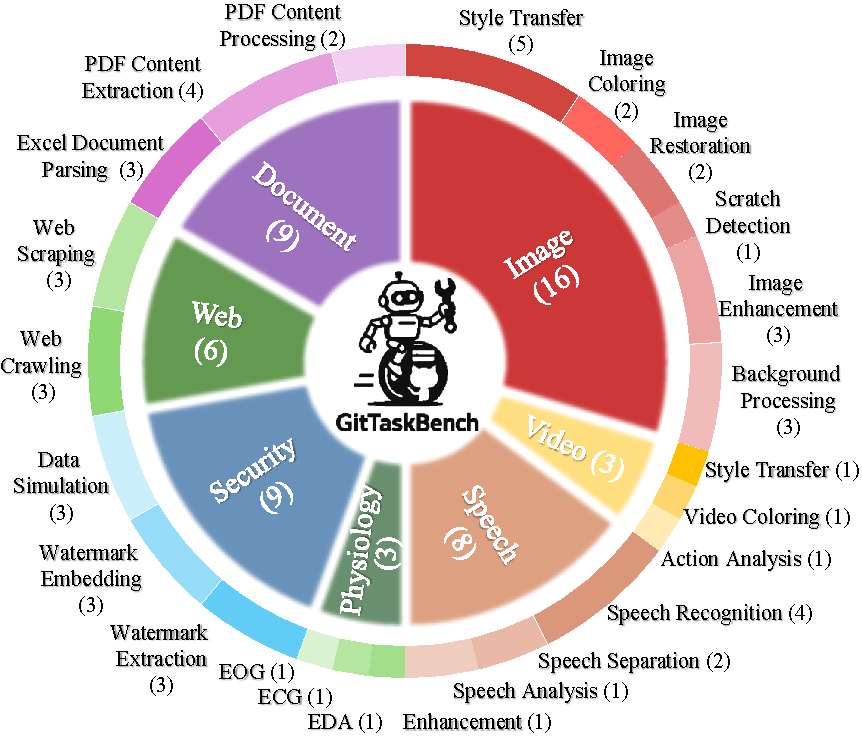
\includegraphics[width=1\linewidth]{images/Domain_v4_50.pdf}
    \caption{Overview of Task Domains in GitTaskBench.}
    \label{fig:datasets}
\end{figure}

\subsection{Task and Repository Selection}		

We began by \textbf{identifying the target domains} through extensive literature reviews, deep LLM-driven research, and consultation with domain experts, combining these insights with practical, everyday experience. For each domain, we \textbf{selected subdomains} that mirror frequent user needs, including a broad spectrum of modalities. 
We prioritized \textit{tasks that are non-trivial}, \textit{typically requiring the integration or reuse of existing tools or codebases}, to ensure that benchmarks are both meaningful and challenging for code agents. 
\textbf{Human completion time} for these tasks ranged up to three hours, averaging \textbf{1.34 hours} per task (see Appendix A).

For each domain, we run targeted deep researches (prompts in Appendix C to \textbf{locate suitable GitHub repos}. Candidates must (1) be Python-based, (2) have $\ge 50$ stars with activity in the past five years (including issue updates), and (3) provide ready-to-use weights and a simple setup. We then inspect key statistics like stars, forks, license, commit history, and manually verify functionality. 
The resulting set formed the pool of potential repositories.

\textit{Task and repository selection was iterative and tightly coupled}—repository capabilities and task requirements were refined in parallel, with each informing the other. When a promising repository was identified, we would \textbf{expand potential task formulations} around its core features. 

Summary statistics of GitTaskBench are presented in Table~\ref{tab:gitaskbench_stats}. 
Figure~\ref{fig:datasets} illustrates the features of each domain.
% Covering multiple modalities, 
GitTaskBench supports both data generation and analysis-oriented objectives. 
See Appendix A for details. 

\subsection{Completeness Verification}
Following the \textbf{Repository Selection} phase, each chosen repository undergoes a stringent \textbf{Completeness Verification}. 
In this human-driven stage, experts follow the repository’s documented instructions, performing tasks exactly as an agent would, ensuring both \textbf{a 100\% human success rate and outputs that satisfy all task requirements}. This process confirms that the repository is fully operational and free of hidden obstacles that could hinder execution.

The verification process includes: Checking for essential \textit{dependencies}, such as \texttt{requirements.txt} or \texttt{package.json};
Confirming the availability of key \textit{configuration} files, like \texttt{config.yaml} or \texttt{setup.py};
Ensuring that the \textit{required datasets} and \textit{pre-trained models} are publicly accessible and properly formatted.

If any required resources are gated or instructions are only available via external links, we supplement the repository by downloading relevant files and inlining essential documentation into the \texttt{README.md}, ensuring all information needed for task execution is completely \textbf{self-contained}. 


\begin{figure*}[t]
    \centering
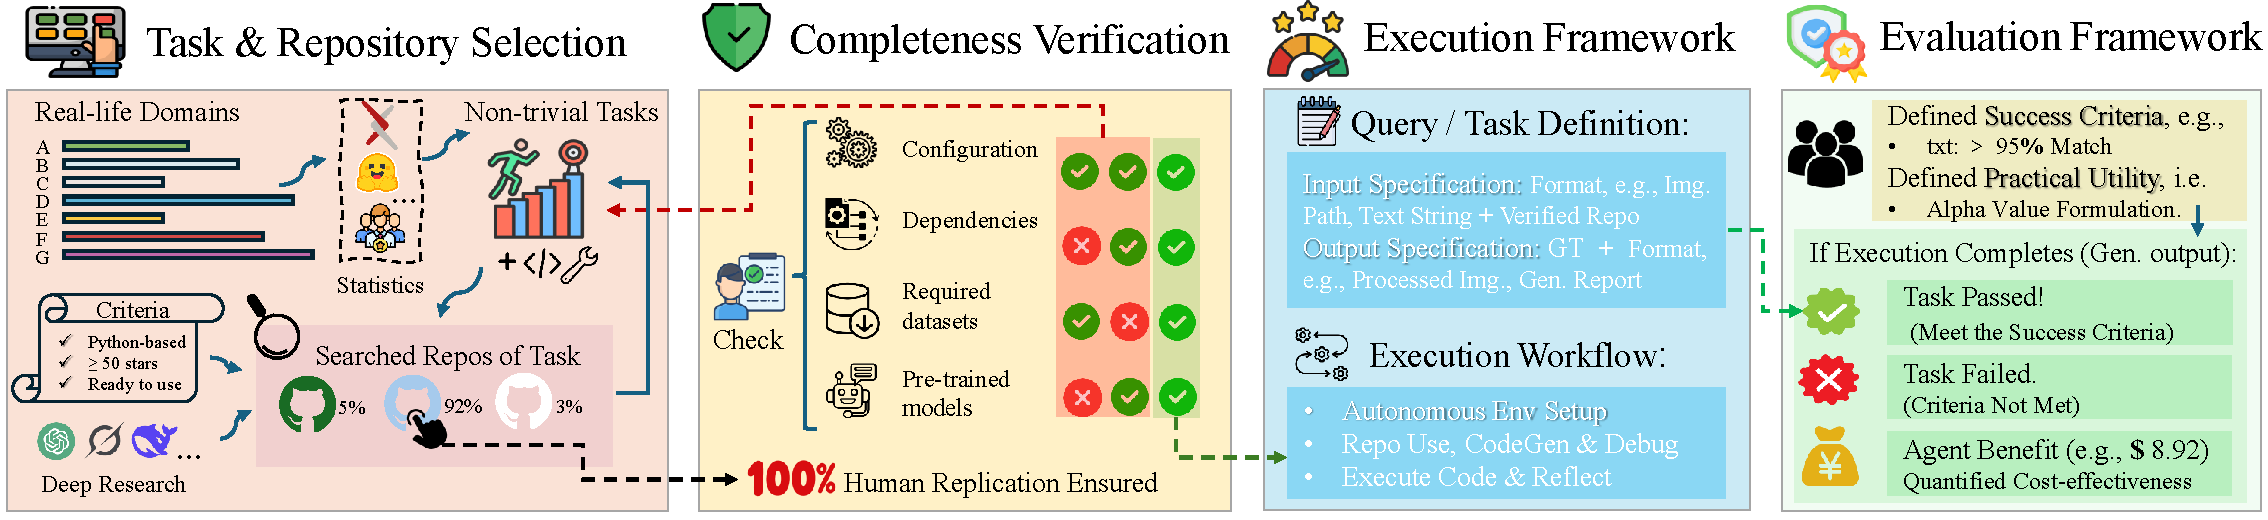
\includegraphics[width=1\textwidth]{images/Benchmark_Construction.pdf}
    \caption{Overview of the GitTaskBench Data Curation and Processing Pipeline.}
    \label{fig:pipeline_diagram}
\end{figure*}



\subsection{Execution Framework Design}
%
To evaluate code agents in realistic and repository-leveraging contexts, we design an execution framework that integrates structured task formulation, automated execution, and output verification. This framework not only tests agents’ capabilities for understanding and utilizing existing codebases but also ensures reproducibility and automation throughout the evaluation process.

\textbf{Task Formulation.} We meticulously define each task, specifying the expected input format (e.g., image path, text string) and the desired output format (e.g., processed image, generated report), ensuring clarity in task goals and reducing ambiguity in prompt interpretation. A single repository may host multiple distinct tasks, each with its clear definition.

\textbf{Agent Inputs and Expected Outputs.} The framework provides the agent with two inputs: a GitHub repository and a task definition prompt. Unlike conventional code generation settings that require only code snippets, our framework emphasizes end-to-end functionality. Agents are expected to return the final task-specific output, which could be a file, text, or visual result, depending on the task requirements. 


\textbf{Execution Workflow.}
Agents are evaluated on their ability to autonomously solve tasks in the multi-stage process: 
\textit{(1) Repository Understanding:} Agents not just read the repository's code, but analyze its structure, dependencies, and available functionalities, often leveraging entry-point documentation such as \texttt{README.md} and selectively parsing key source files.
\textit{(2) Code Generation or Modification:} Based on their understanding and the task definition, agents generate new scripts or adapt existing files to fulfill the task.
\textit{(3) Environment Setup:} Agents are expected to construct the required execution environment, including issuing installation commands (e.g., \texttt{pip install -r requirements.txt}) and resolving dependency issues.
\textit{(4) Code Execution:} The generated or modified code is executed automatically in the sandbox, directly assessing the agent's ability to produce runnable and correct solutions.


\subsection{Evaluation Framework}
To support automated, practical, and cost-benefit evaluation, we introduce the following metrics, which are implemented through hand-verified custom-built test scripts.

\textbf{Execution Completion Rate (ECR).} ECR measures the proportion of cases where the agent successfully executes the target code repository and generates outputs in an acceptable format (e.g., \texttt{.jpg} or \texttt{.png} for image processing tasks). This metric reflects the agent's compatibility with the code repository and its basic operational capability. It ensures that: (1) the output file(s) exist, (2) the output file(s) are not empty, and (3) the output format can be correctly processed by the testing scripts.

\textbf{Task Pass Rate (TPR).} TPR quantifies the agent's actual performance quality in task completion. It is determined by formulating evaluation test functions and defining concrete success and failure criteria using established metrics tailored to each task, drawing on standards recognized within the domain developer community. TPR requires the agent's outputs to satisfy predefined quality standards, such as functional correctness, result completeness, or achieving specific task objectives. For example, in speech enhancement tasks, success might be defined by achieving a \textbf{PESQ $\ge 2.0$} (indicating acceptable perceptual quality) and a \textbf{SNR $\ge 15 dB$} (suggesting good suppression of noise). Tasks failing to meet these thresholds are marked as failures.


% \textbf{By Automated Test Scripts.}
\textbf{Both of the above metrics are evaluated using hand-crafted test scripts.} Additionally, we streamlined the benchmarking process so that all tasks can be automatically assessed with a single shell command. The evaluation outputs a clear “Process” and “Result” status (success or failure), along with detailed “Comments” explaining the outcome—such as which metric exceeded a threshold, which criterion caused failure, or any error messages encountered during execution.
See Appendix~A for example test results.

 
\textbf{Alpha Practical Value Assessment.} We introduce a new perspective for evaluating LLM agents by incorporating market-driven cost considerations. While technical metrics like ECR and TPR are essential, they overlook cost-effectiveness. High technical performance alone does not guarantee practical utility—an agent is only valuable if it completes tasks more cheaply than human labor, without sacrificing quality. In practice, agents incur tangible operational costs, like API fees for proprietary LLMs or hardware expenses for open-source solutions. 
%
We estimate the economic value of agent-completed tasks by quantifying potential cost savings, efficiency gains, and market impact from automation and scalability of these tasks. 
Accordingly, we propose the \textbf{\(\boldsymbol{\alpha}\)-score}, a value-based metric defined as the average net benefit generated by the agent across tasks:

\begin{equation}
\alpha=\frac{1}{n} \sum_{i=1}^{n} \left [(T\times MV\times Q)- C \right ] 
\end{equation}
where $n$ is the number of tasks in the evaluated area; $T$ is a binary indicator of task success (1 if the agent successfully executes the target code repository, 0 otherwise), consistent with the definition of ECR; $MV$ represents the estimated, prevailing market value of the task if completed by a human; $Q$ is a quality factor (ranging from 0 to 1) that measures how closely the agent’s output approximates the groundtruth produced by a human executing the same code repository; and $C$ denotes the agent’s total operational cost, which is approximated here as the API cost. The resulting \textbf{\(\boldsymbol{\alpha}\)-score} clearly reflects the economic viability and gains of the agent-based automation approach across the evaluated areas.


\textbf{Human Check.} 
% A critical component of quality assurance involves human expert review along the dimension: 
Experts compare the automatically generated assessment of a repository/task with their own manual execution and evaluation, identifying any discrepancies or inconsistencies. For generating the groundtruth, humans can interpret the task requirements and iteratively adjust repository parameters to obtain the best possible output. 

Because this expert-guided result provides a reliable upper bound on quality, we derive \(Q\) through human assessment. Five raters independently compare each agent output with the groundtruth and assign it to one of five levels—far below human (\texttt{0}), large gap (\texttt{0.25}), moderate gap (\texttt{0.50}), near parity (\texttt{0.75}), or indistinguishable from/better than human (\texttt{1}). The level chosen by the majority is recorded as the final \(Q\) value. 
\(MV\) is drawn from publicly listed freelance fees on the platforms 
% (like Upwork, Fiverr, and Freelancer) \footnote{ Upwork: https://www.upwork.com/}\footnote{ Fiverr: https://www.fiverr.com}\footnote{ Freelancer: https://www.freelancer.com}
\cite{upwork, fiverr, freelancer}
for similar deliverables—for example, roughly \$10 per restored photo on Fiverr—providing a consistent task-level benchmark for the \(\alpha\)-score. 
Details on estimated market values for all GitTaskBench tasks, application cases, and analysis are provided in Appendix D.



\section{Experiments} % results

\subsection{Setup}

\renewcommand{\floatpagefraction}{.15}
\renewcommand{\textfraction}{.1}
% \renewcommand{\arraystretch}{1.2}  % 拉高单元格高度
\begin{table*}[!t]
\centering
\small
\renewcommand{\arraystretch}{1.1}
\begin{tabular}{llccccc}
\toprule
\textbf{Framework} & \textbf{LLM} & 
\textbf{ECR (\%) $\uparrow$} & 
\textbf{TPR (\%) $\uparrow$} & 
\textbf{Input Tokens (k) $\downarrow$} & 
\textbf{Output Tokens $\downarrow$} & 
\textbf{Cost (\$) $\downarrow$} \\
\midrule
\multirow{4}{*}{Aider}
& \cellcolor{gray!4}GPT-4o       & \cellcolor{gray!4}5.56         & 
\cellcolor{gray!4}1.85         & 
\cellcolor{gray!4}10.67        & \cellcolor{gray!4}\textbf{492.67}     & \cellcolor{gray!4}0.0316            \\
& \cellcolor{gray!8}GPT-4.1      & \cellcolor{gray!8}11.11        & \cellcolor{gray!8}7.41         & \cellcolor{gray!8}14.83        & \cellcolor{gray!8}734.17             & \cellcolor{gray!8}0.0355           \\
& \cellcolor{gray!12}Claude 3.5    & \cellcolor{gray!12}\underline{16.67}        & \cellcolor{gray!12}\underline{12.96}        & \cellcolor{gray!12}\textbf{7.48} & \cellcolor{gray!12}\underline{534.00}  & \cellcolor{gray!12}\underline{0.0304} \\
& \cellcolor{gray!12}DeepSeekV3   & \cellcolor{gray!12}\textbf{20.37}        & \cellcolor{gray!12}\textbf{16.67}        & \cellcolor{gray!12}\underline{7.51} & 
\cellcolor{gray!12}599.64         & \cellcolor{gray!12}\textbf{0.00269} \\

\midrule
\multirow{8}{*}{SWE-Agent}
& \cellcolor{gray!8}GPT-4o       & \cellcolor{gray!8}17.58        & 
\cellcolor{gray!8}10.19        & \cellcolor{gray!8}275.53       & \cellcolor{gray!8}1282.70            & \cellcolor{gray!8}0.778            
\\
& \cellcolor{gray!20}GPT-4.1      
& \cellcolor{gray!20}38.89        
& \cellcolor{gray!20}\underline{31.48}        
& \cellcolor{gray!20}301.11       
& \cellcolor{gray!20}2098.33            
& \cellcolor{gray!20}0.661            
\\
& \cellcolor{gray!16}o3-mini      & \cellcolor{gray!16}25.93 & \cellcolor{gray!16}20.37 &
\cellcolor{gray!16}\underline{158.45} &
\cellcolor{gray!16}\textbf{215.20} & 
\cellcolor{gray!16}\underline{0.175} 
\\
& \cellcolor{gray!16}Claude 3.5    & \cellcolor{gray!16}\underline{41.67} & \cellcolor{gray!16}22.23       & \cellcolor{gray!16}455.34       & \cellcolor{gray!16}943.30             & \cellcolor{gray!16}1.38          
\\
& \cellcolor{gray!32}Claude 3.7    & \cellcolor{gray!32}\textbf{64.81} & \cellcolor{gray!32}\textbf{42.59}       & \cellcolor{gray!32}552.79       & \cellcolor{gray!32}807.63             & \cellcolor{gray!32}1.67            
\\
& \cellcolor{gray!12}DeepSeekV3   & 
\cellcolor{gray!12}18.52        & 
\cellcolor{gray!12}12.04        & 
\cellcolor{gray!12}412.65       & 
\cellcolor{gray!12}1649.82            & \cellcolor{gray!12}\textbf{0.113}          
\\
& \cellcolor{gray!4}Qwen3-32b$^{*}$        & 
\cellcolor{gray!4}7.41            & 
\cellcolor{gray!4}3.70            & 
\cellcolor{gray!4}1445.97            & 
\cellcolor{gray!4}2405.00                  & 
\cellcolor{gray!4}-             
\\
& \cellcolor{gray!12}Qwen3-32b$^{*\dagger}$    
& \cellcolor{gray!12}16.67        
& \cellcolor{gray!12}11.11        
& \cellcolor{gray!12}\textbf{124.15}  
& \cellcolor{gray!12}\underline{559.11}          
& \cellcolor{gray!12}-                
\\
& \cellcolor{gray!12}Llama3.3-70b$^{*}$        & 
\cellcolor{gray!12}25.83            & 
\cellcolor{gray!12}18.52            & 
\cellcolor{gray!12}397.03            & 
\cellcolor{gray!12}1985.64                  & 
\cellcolor{gray!12}-              
\\

\midrule
\multirow{12}{*}{OpenHands}
& \cellcolor{gray!12}GPT-4o       & 
\cellcolor{gray!12}21.30        & 
\cellcolor{gray!12}14.82        & 
\cellcolor{gray!12}760.53       & 
\cellcolor{gray!12}3990.31            & 
\cellcolor{gray!12}1.94             
\\
& \cellcolor{gray!32}GPT-4.1      & \cellcolor{gray!32}\underline{55.56} & \cellcolor{gray!32}\underline{42.59} & \cellcolor{gray!32}465.94   & \cellcolor{gray!32}\underline{1535.47}            & \cellcolor{gray!32}\textbf{0.942} 
\\
& \cellcolor{gray!16}o3-mini      & \cellcolor{gray!16}29.63 & \cellcolor{gray!16}22.22 &
\cellcolor{gray!16}2523.53 &
\cellcolor{gray!16}183637.53 & 
\cellcolor{gray!16}3.58 
\\
& \cellcolor{gray!32}Claude 3.5    & 
\cellcolor{gray!32}53.70        & 
\cellcolor{gray!32}40.74        & 
\cellcolor{gray!32}2858.00      & 
\cellcolor{gray!32}24929.47           & 
\cellcolor{gray!32}8.95            
\\
& \cellcolor{gray!36}Claude 3.7    & \cellcolor{gray!36}\textbf{72.22} & \cellcolor{gray!36}\textbf{48.15} & \cellcolor{gray!36}9501.25 & 
\cellcolor{gray!36}85033.05  & 
\cellcolor{gray!36}29.8        
\\
& \cellcolor{gray!24}Gemini-2.5-pro   & 
\cellcolor{gray!24}51.85        & 
\cellcolor{gray!24}35.19        & 
\cellcolor{gray!24}760.88       & 
\cellcolor{gray!24}35173.29     & 
\cellcolor{gray!24}2.18   
\\
& \cellcolor{gray!20}DeepSeekV3   & 
\cellcolor{gray!20}45.37        & 
\cellcolor{gray!20}26.85        & 
\cellcolor{gray!20}4717.78      & 
\cellcolor{gray!20}31957.67           & 
\cellcolor{gray!20}\underline{1.31}  
\\
& \cellcolor{gray!4}Qwen3-8b$^{*}$        & \cellcolor{gray!4}1.85       
& \cellcolor{gray!4}1.85        
& \cellcolor{gray!4}846.26    
& \cellcolor{gray!4}2045.00             
& \cellcolor{gray!4}-                
\\
& \cellcolor{gray!8}Qwen3-14b$^{*}$        
& \cellcolor{gray!8}11.11        
& \cellcolor{gray!8}5.56       
& \cellcolor{gray!8}339.42      
& \cellcolor{gray!8}2540.17             
& \cellcolor{gray!8}-                
\\
& \cellcolor{gray!20}Qwen3-32b$^{*}$    
& \cellcolor{gray!20}35.19        
& \cellcolor{gray!20}25.93        
& \cellcolor{gray!20}591.02   
& \cellcolor{gray!20}2097.89         
& \cellcolor{gray!20}-                
\\
& \cellcolor{gray!20}Qwen3-32b$^{*\dagger}$    
& \cellcolor{gray!20}44.44        
& \cellcolor{gray!20}29.63        
& \cellcolor{gray!20}\underline{208.00}     
& \cellcolor{gray!20}8755.35         
& \cellcolor{gray!20}-                
\\
& \cellcolor{gray!12}Llama3.3-70b$^{*}$    
& \cellcolor{gray!12}27.78        
& \cellcolor{gray!12}20.37        
& \cellcolor{gray!12}\textbf{132.69}      
& \cellcolor{gray!12}\textbf{872.93}          
& \cellcolor{gray!12}-            
\\
\bottomrule
\end{tabular}
\caption{
Performance Comparison of Different Frameworks and LLMs on GitTaskBench. 
Bold values indicate the best among all models for each metric; underlined values denote the second-best.
The best-performing row for each metric is highlighted. 
All token values are rounded to two decimal places. 
\texttt{$^*$} means our self-deployed model. 
\texttt{$^\dagger$}: with think mode.
% \texttt{$^\ddagger$} denotes the model in think mode.
}
\label{tab:git-task-perf}
\end{table*}



We evaluate three representative open-source frameworks that are capable of handling our benchmark tasks: \textbf{Aider} \cite{aider2025}, \textbf{OpenHands} \cite{wang2025openhands}, and \textbf{SWE-Agent} \cite{swe-agent}. 
% To the best of our knowledge, these are the only open-source frameworks capable of tackling the complex, comprehensive tasks in our benchmark. 
% 这些是经过我们调研唯一能完成我们benchmark这类复杂综合的开源框架。
% —on several advanced LLMs. 
% These frameworks are designed to mimic the workflow of human programmers, autonomously analyzing and interacting with code repositories.  
% Each agent executes Python code and bash commands in a Linux sandbox without pre-configured environments. 
Execution configurations and framework settings are detailed in Appendix B.
In terms of \textbf{LLMs,}
we evaluate multiple advanced models, including the closed-source GPT-4o-2024-08-06 \cite{gpt4o}, GPT-4.1 \cite{gpt41}, and o3-mini (medium reasoning effort) \cite{o3mini}, Claude-3-5-sonnet-20241022 \cite{claude35sonnet} and Claude-3-7-sonnet-20250219 \cite{claude37sonnet}, Gemini-2.5-pro~\cite{gemini25_report}, as well as the open-source DeepSeek-V3-0324 \cite{liu2024deepseekV3}, Qwen3-8b, 14b, 32b \cite{yang2025qwen3} and Llama3.3-70b \cite{llama3.3}. 
For robustness, all reported results are averaged over two independent runs under identical settings.


\subsection{Comparative Analysis}

Different framework–LLM pairings exhibit substantial performance disparities, affecting both effectiveness (ECR, TPR) and efficiency (token usage, cost, API calls).

\textbf{OpenHands achieves the best overall performance across all frameworks.}
As shown in Table~\ref{tab:git-task-perf}, \textbf{(1)} OpenHands+Claude 3.7 delivers the best results (ECR 72.22\%, TPR 48.15\%) among all evaluated settings. \textbf{(2)} With the same LLM, OpenHands consistently outperforms Aider and SWE-Agent, likely due to its robust code execution capabilities and more proactive and explorative strategies. 

\textbf{OpenHands offers higher success rates, while SWE-Agent balances moderate cost and efficiency as a lower-cost alternative.}
SWE-Agent consistently uses fewer tokens than OpenHands when paired with top-performing closed-source models, indicating stronger control over context token usage. 
Meanwhile, Aider+DeepSeek V3 yields the lowest cost ($<$ \$0.003) with reasonable output.

\textbf{GPT-4.1 is more cost-efficient than Claude.}  
\textbf{(1)} In SWE-Agent, Claude 3.7 leads but costs 2x more than 2nd-place GPT-4.1. 
\textbf{(2)} Under OpenHands, GPT-4.1  also delivers the 2nd-best ECR/TPR at just 1/10 or 1/30 of Claude's cost. 


\textbf{Open-source models generally underperform closed ones.} But Qwen3-32B (with think mode) is impressive---reaching up to 60\% of top closed Claude3.5's performance with far lower token usage. In contrast, Gemini 2.5 Pro underwhelms in think mode, likely due to the added context burden in our long, token-heavy, complex real-world tasks.


These findings highlight \textit{trade-offs between performance, cost, and interaction complexity} when choosing agents---framework and model combinations.
Next, we drill down into domain-specific performance, as visualized in Figure~\ref{fig:ratio-domain}. 

\textbf{Agents perform notably better on purely textual tasks compared to multimodal, model-based tasks.}
Specifically, \textbf{(1) }most agents process office documents effectively, such as parsing Excel files with \texttt{Eparse} or splitting PDFs using \texttt{PyPDF}. That is because these workflows typically require reading simple wrapper scripts that import the library API. 
\textbf{(2)} In contrast, multimodal tasks, especially in image or speech processing domains, mainly involve model-based processing and prediction and thus demand much deeper competence. 
For example, removing image scratches with \texttt{DeScratch} entails installing multiple dependencies, downloading pretrained weights, and configuring runtime arguments---all of which require a nuanced understanding of the repository’s build and execution process. 

Current agents often struggle with such complex workflows, suggesting that \textbf{future work should focus on richer codebase comprehension and automated environment management} beyond what a simple \texttt{README} scan provides.


\begin{figure*}
    \centering   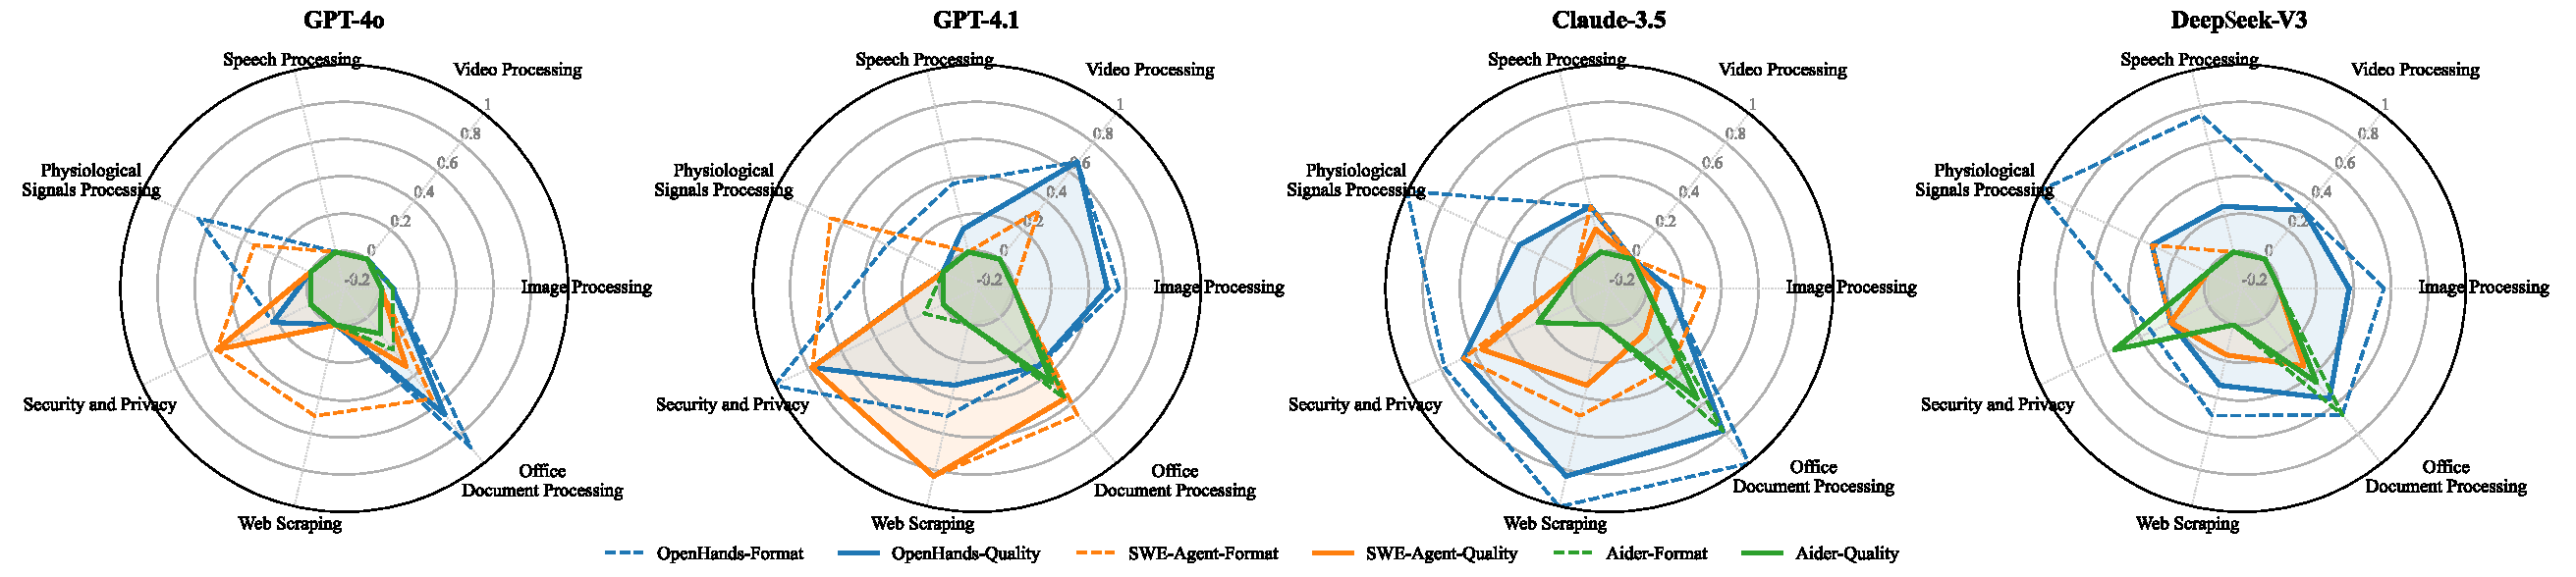
\includegraphics[width=1\linewidth]{images/ratio_domain.pdf} 
    \caption{Performance Evaluation of GPT-4o, GPT-4.1, Claude 3.5, DeepSeek V3  across Different Task Domains.} 
    \label{fig:ratio-domain}
\end{figure*}

\subsection{Sensitivity Analysis to Configuration Changes}

\begin{figure}[t]
    \centering   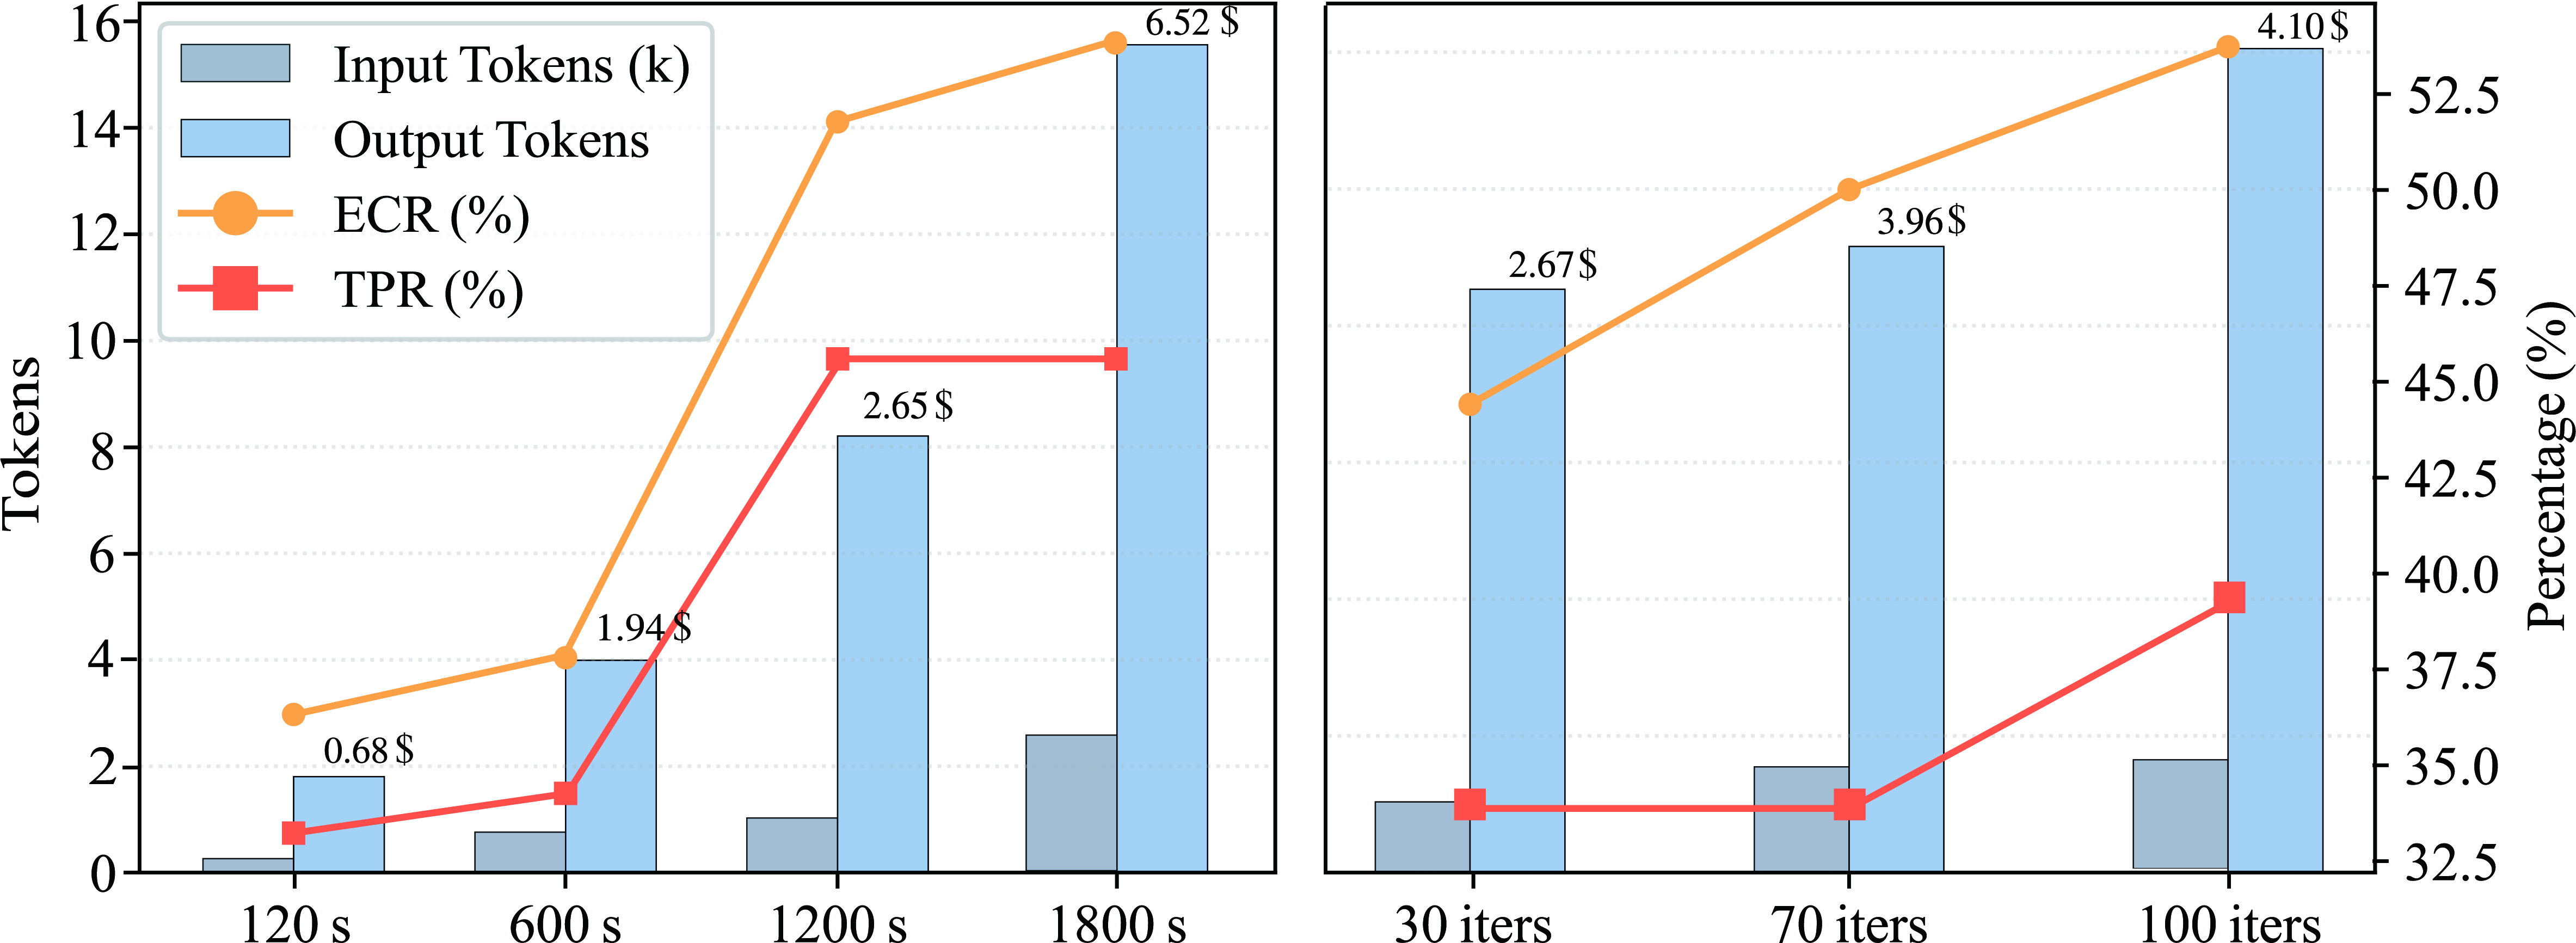
\includegraphics[width=1\linewidth]{images/parameter.jpg}
    \caption{Effect of Timeout (max\_iteration = default) and Max Iteration (timeout = 600s) on OpenHands (GPT-4o).}
    \label{fig:openhands-gpt4o-hyperparam}
\end{figure}


Since OpenHands consistently outperformed SWE-Agent overall, we examined how its key hyperparameters affect performance. Notably, GPT-4o with OpenHands lagged behind despite strong overall results, with execution traces revealing \textit{frequent failures from environment setup errors and flawed code generation}. To clarify these issues, we tested two critical hyperparameters. \texttt{timeout}: Maximum time per iteration. \texttt{max\_iteration}: Total environment interactions allowed.
Performance variation is in Table~\ref{fig:openhands-gpt4o-hyperparam}.

Results show that more generous settings significantly boost performance. Increasing the \texttt{timeout} (from 120s to 1800s) raises both ECR and TPR, but also incurs more tokens, indicating that \textbf{environment setup may be the primary time-consuming step in repurposing repositories}. Similarly, increasing \texttt{max\_iteration} (from 30 to 100) consistently improves ECR and TPR, suggesting that \textbf{more interaction rounds could help mitigate errors within reasonable limits}. 
Overall, these findings underscore the importance of tuning both interaction depth and time budgets to balance effectiveness and computational efficiency. 


\subsection{Practical Benefits Analysis}

\begin{figure}[t]
    \centering
    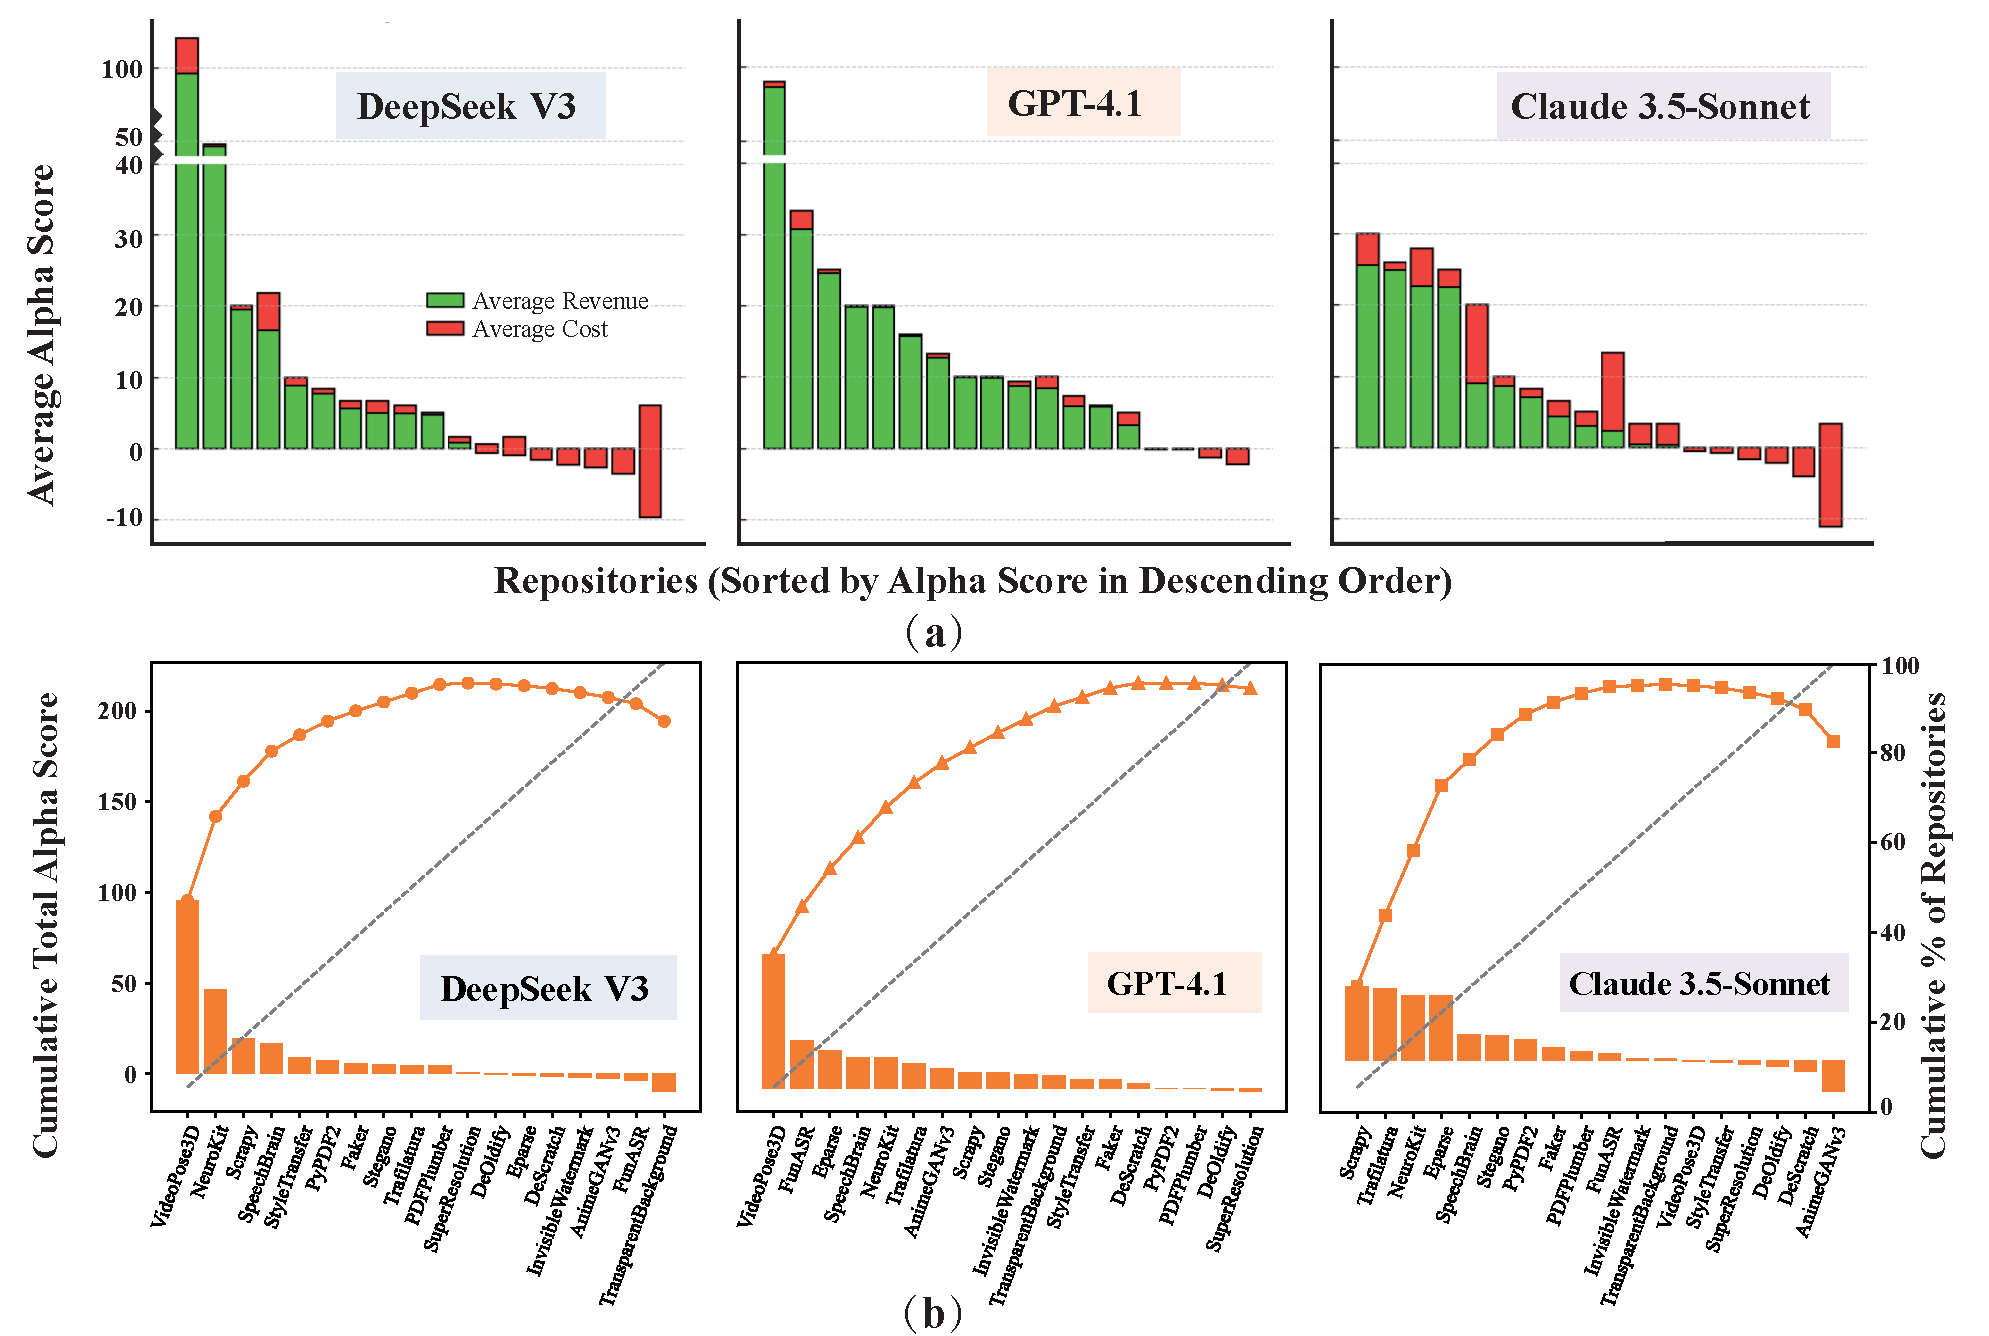
\includegraphics[width=1\linewidth]{images/alpha.pdf}
    \caption{The $\alpha$ per Repository (a) and Pareto Curves (b).}
    \label{fig:alpha_results}
\end{figure}


Given OpenHands’ strong overall performance, we select it as the evaluation backbone for estimating the practical value of the three most cost-effective models.
% : DeepSeek V3, GPT-4.1, and Claude 3.5. 
We treat each repository as a domain, capturing agents’ domain-specific applicability and their ability to leverage the code. 
For each repository, we computed \(\alpha\)-score by averaging net gains of all \(n\) tasks executed with that repository, as defined in Eq~(1). 
% ,(e.g., \(n{=}5\) for \texttt{SpeechBrain}), as defined in Eq~(1). 

Figure~\ref{fig:alpha_results} (a) presents the \(\alpha\) score (green revenue minus red cost) of each repository, facilitating a direct cost-benefit comparison across models and repositories. 
Figure~\ref{fig:alpha_results} (b) displays the Pareto curves, illustrating how each model’s total alpha is distributed across repositories. The dashed 45-degree reference line represents a perfectly even distribution: if the cumulative alpha curve rises steeply and surpasses the diagonal early, it means just a few repositories contribute most of the total benefit (high concentration). In contrast, if a curve close to the diagonal means alpha is more evenly spread across repositories. This directly reveals the difference in benefit concentration for each model. 

\textbf{Expensive tasks are always profitable if completed by the agent, while cheap tasks require careful cost control.}
Repositories with intrinsically high human market value (\(MV\)), like \texttt{VideoPose3D}, \texttt{FunASR}, and \texttt{NeuroKit}, yield the largest positive \(\alpha\) when agents succeed. Low-\(MV\) image-processing tasks (\(MV\!\approx\$5\text{--}10\)) often produce negative \(\alpha\) once the agent’s average cost exceeds \$1--2. This pattern underscores the importance of controlling operational costs for tasks with limited commercial potential.

DeepSeek V3 delivers the highest overall benefit and best cost–performance for most repositories. 
GPT-4.1’s performance is more consistent and robust across scenarios, with fewer large losses. 
Claude 3.5 has the most dispersed returns, excelling at information extraction but being cost-sensitive on compute-intensive vision tasks.

The $\alpha$ score captures meaningful distinctions that technical metrics (ECR/TPR) alone may miss, emphasizing the need to align agent deployment with task-specific economic profiles. Details are provided in Appendix D. 


\subsection{Error Analysis}

To better understand the challenges in such repository-centric tasks, we studied execution errors encountered across various agents. We grouped all errors into five types: \textbf{E1, }Environment-Setup; \textbf{E2, }Workflow Planning; \textbf{E3, }Repository Comprehension; \textbf{E4: }Runtime; and \textbf{E5: }Failures to Follow Instructions. Case studies are shown in Appendix F.
% All success and failure case studies are clearly shown in Appendix F.

\begin{figure}[t]
    \centering
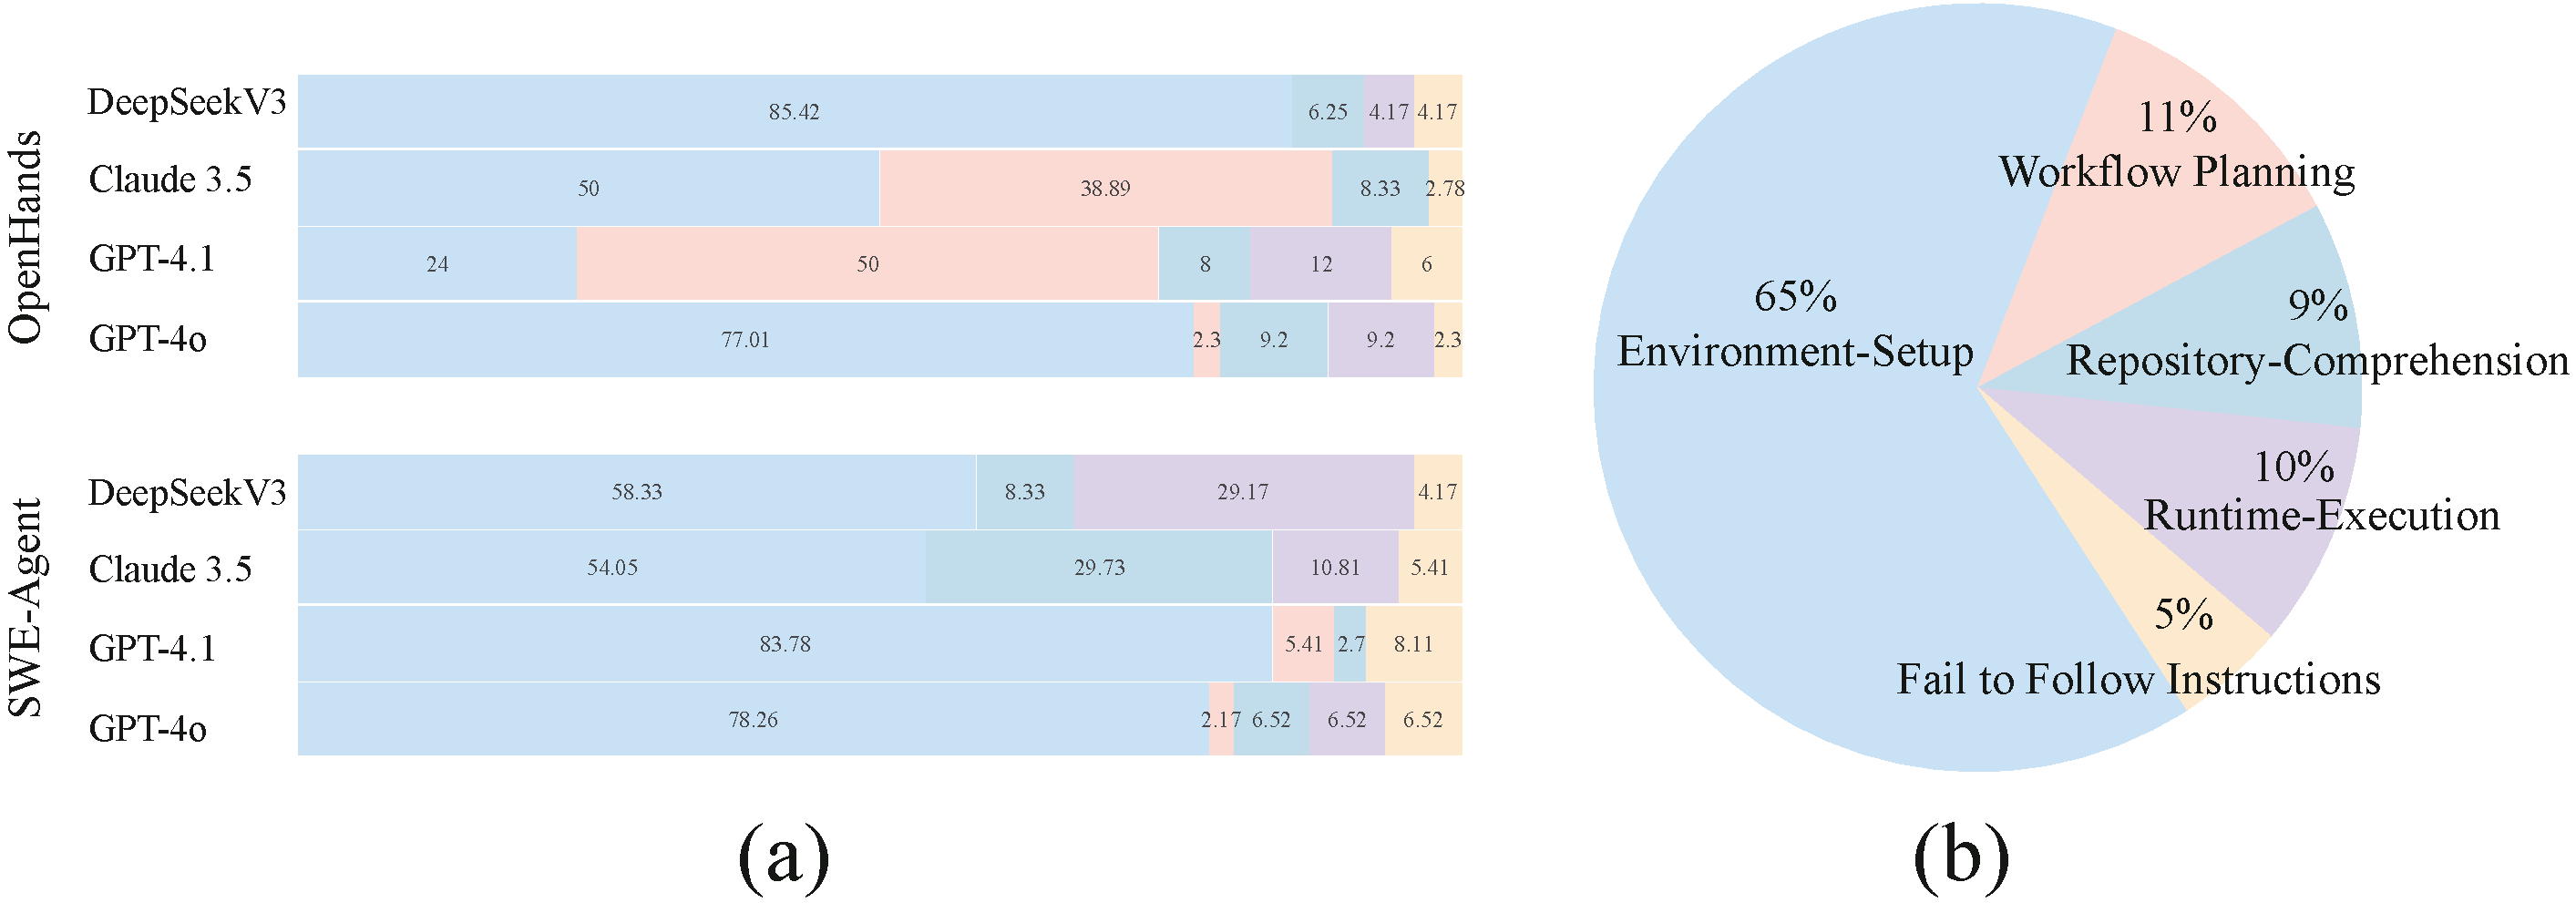
\includegraphics[width=1\linewidth]{images/error_analysis_v4.pdf}
    \caption{Distribution of Errors per Agent (a) and Overall Error Statistics (b).}
    \label{fig:enter-label}
\end{figure}

As summarized in Figure~\ref{fig:enter-label} (b), E1 errors were the most common, constituting 65.04\% of all failures. These usually came from dependency conflicts, missing binary wheels, or absent system-level libraries. Notably, env setup doesn’t improve results but causes most failures---showing its unavoidable importance in real-world agent applications. E2 errors mainly reflected agents' inability to orchestrate execution sequences or their stagnation at setup stages. E3 errors occurred when agents misidentified entry-point scripts or misused APIs within repositories. E4 errors involved premature termination due to system freezes, timeouts, or interrupts (\texttt{Ctrl+C}). E5 errors, the least frequent, included things like wrong file naming, incorrect output formats,  missing deliverables, or solving the task without using the repository as required. 
Check Appendix F for examples of each.

We compared errors across agents/models and found similar weaknesses regardless of architecture (see Figure~\ref{fig:enter-label} (a)). Key improvements could be summarized as: robust dependency management, enhanced execution planning, deeper repo comprehension, smarter resource handling during runtime, and rigorous instruction following---all crucial for more reliable and effective real-world agent performance.



\section{Conclusion}
We introduced GitTaskBench, a benchmark for evaluating agents’ ability to leverage repository code for complex task solving. With carefully curated tasks, thoroughly reviewed repositories, and practical automated evaluation, GitTaskBench sets a new standard for assessing real-world agent utility. We hope this benchmark drives greater focus on repository utilization for everyday, non-technical challenges and encourages economic value-driven agent applications.



\bibliography{aaai2026}


\appendix
\appendix
\section*{Appendices}
\section*{A. Details of GitTaskBench}\label{appendix:gittaskbench}

\subsection*{Tasks.}
The GitTaskBench benchmark includes a wide range of real-world tasks spanning 7 domains and 24 subdomains. The statistics of tasks by Domain are shown in the Table \ref{tab:Tasks by Domain}.
The largest category is Image Processing, encompassing 16 tasks (29.63\%), which include style transfer (9.26\%), image enhancement (5.56\%), background processing (5.56\%), image coloring (3.70\%), restoration (3.70\%), and scratch detection (1.85\%). Speech Processing ranks second with 8 tasks (14.81\%), covering speech recognition (7.41\%), separation (3.70\%), enhancement (1.85\%), and analysis (1.85\%). Security and Privacy also accounts for 9 tasks (16.67\%) evenly divided into 3 data simulation tasks, 3 watermark embedding tasks, and 3 watermark extraction tasks. The Office Document Processing domain contributes another 9 tasks (16.67\%), divided into PDF content extraction (7.41\%), Excel document parsing (5.56\%), and PDF processing (3.70\%). Other domains include Web Scraping (6 tasks, 11.12\%), Video Processing (3 tasks, 5.55\%), and Physiological Signal Processing (3 tasks, 5.55\%)---the latter dealing with electrodermal activity, electrocardiogram, and electrooculogram data analysis.


\begin{table*}[ht]
\centering
\renewcommand{\arraystretch}{1.2}
\resizebox{0.88\textwidth}{!}{%
\begin{tabular}{l|l|c}
\hline
% \hline
\textbf{Domain (Task Count, \%)} & \textbf{Subdomain} & \textbf{Percentage (\%)} \\
\hline
\multirow{6}{*}{Image Processing (16, 29.63\%)}
& Style Transfer & 9.26 \\
& Image Coloring & 3.70 \\
& Image Restoration & 3.70 \\
& Scratch Detection & 1.85 \\
& Image Enhancement & 5.56 \\
& Background Processing & 5.56 \\
\hline
\multirow{3}{*}{Video Processing (3, 5.55\%)}
& Video Action Analysis & 1.85 \\
& Style Transfer & 1.85 \\
& Video Coloring & 1.85 \\
\hline
\multirow{4}{*}{Speech Processing (8, 14.81\%)}
& Speech Recognition & 7.41 \\
& Speech Separation & 3.70 \\
& Speech Enhancement & 1.85 \\
& Speech Analysis & 1.85 \\
\hline
\multirow{3}{*}{Physiological Signal Processing (3, 5.55\%)}
& Electrodermal Activity Data Analysis & 1.85 \\
& Electrocardiogram Data Analysis& 1.85 \\
& Electrooculogram Data Analysis& 1.85 \\
\hline
\multirow{3}{*}{Security and Privacy (9, 16.67\%)}
& Data Simulation & 5.56 \\
& Watermark Embedding & 5.55 \\
& Watermark Extraction & 5.56 \\
\hline
\multirow{2}{*}{Web Scraping (6, 11.12\%)}
& Web Scraping & 5.56 \\
& Web Crawling & 5.56 \\
\hline
\multirow{3}{*}{Office Document Processing (9, 16.67\%)}
& Excel Document Parsing & 5.56 \\
& PDF Content Extraction & 7.41 \\
& PDF Content Processing & 3.70 \\
\hline
\textbf{Overall} & \textbf{Total} & \textbf{100.00} \\
\hline
% \hline
\end{tabular}
}
\caption{Statistics of Tasks by Domain in GitTaskBench}
\label{tab:Tasks by Domain}
\end{table*}



\subsection*{Repositories.}
The repositories included in GitTaskBench span a wide range of codebases, exhibiting considerable diversity in scale, structure, and complexity. For instance, repositories like FunASR and Faker contain over 1,000 files, with more than 3,000 functions and 10,000 function calls, highlighting the massive code volume. Some repositories, such as SpeechBrain and Scrapy, feature extremely high internal connectivity with more than 40,000 function calls and thousands of import dependencies. On average, each repository has over 200 files, 1,200 functions, and nearly 8,600 intra-repository calls, with more than 448,000 tokens per repository. These figures reflect not only the sheer volume of code and modularity but also the highly entangled dependencies and large-scale function interactions present across projects. As such, understanding and effectively leveraging these repositories pose significant challenges for code agents, especially in tasks requiring comprehensive reasoning over multiple modules, imports, and usage patterns. The comprehensive statistics are demonstrated in the Table \ref{tab:appendix-static-analysis}.

The "Manual Reproduction Time" column measures the approximate time, in hours, that a PhD student in computer science needs to fully understand and use each repository to complete its associated tasks. Across the 18 repositories analyzed, this time varies between 0.50 hours and 3.00 hours, with an average of 1.34 hours.
These findings shed light on the complexity of the repositories. Even for highly skilled individuals, such as PhD students, it takes more than an hour on average to comprehend and implement the code effectively. For instance, the VideoPose3D repository stands out, requiring up to 3.00 hours, which emphasizes the challenging nature of its tasks.

This further suggests that working with these repositories is far from straightforward---it’s a significant effort, even for experienced professionals. Beyond that, these results also serve as an important reference point for assessing how well automated systems can manage similarly intricate tasks.


\begin{table*}[htb]
\centering
\renewcommand{\arraystretch}{1.5}
\resizebox{\textwidth}{!}{%
\begin{tabular}{l|rrrrrrrc}
\toprule
\textbf{Repository} & \#\textbf{Files} & \#\textbf{Classes} & \#\textbf{Functions} & \textbf{LOC} & \textbf{Imports} & \textbf{Calls} & \textbf{Tokens} 
&\makecell[c]{\textbf{Manual}\\\textbf{Reproduction Time (h)}}\\
\midrule
AnimeGANv3             & 25   & 7    & 191  & 3540   & 140  & 1465  & 39288  &2.25  \\
DeOldify               & 105  & 280  & 1743 & 15776  & 727  & 7552  & 187418 &2.33 \\
DeScratch              & 64   & 61   & 394  & 9606   & 401  & 3277  & 82321  &2.00 \\
Eparse                 & 13   & 10   & 67   & 1872   & 108  & 380   & 11577  &0.83 \\
Faker                  & 754  & 1130 & 3361 & 351420 & 1879 & 11922 & 2888354 &0.50\\
FunASR                 & 1157 & 1093 & 3843 & 132830 & 6979 & 39459 & 1151842 &2.00\\
InvisibleWatermark     & 7    & 5    & 39   & 575    & 34   & 180   & 4870   &0.50 \\
NeuroKit               & 349  & 2    & 979  & 57270  & 1819 & 11479 & 508910  &1.50\\
PDFPlumber             & 38   & 46   & 441  & 8339   & 413  & 2136  & 66653   &0.50\\
PyPDF2                 & 89   & 152  & 1488 & 50709  & 1226 & 10819 & 491912  &0.67\\
Scrapy                 & 362  & 1144 & 4533 & 67685  & 3660 & 18376 & 536203  &0.67\\
SpeechBrain            & 573  & 736  & 4915 & 207652 & 3799 & 40552 & 1596907 &0.83\\
Stegano                & 25   & 9    & 93   & 2270   & 74   & 510   & 18207   &0.50\\
StyleTransfer          & 7    & 3    & 25   & 747    & 33   & 380   & 8796    &2.17\\
SuperResolution        & 29   & 20   & 208  & 3777   & 158  & 1237  & 32940   &1.67\\
Trafilatura            & 41   & 11   & 437  & 27399  & 686  & 4329  & 397119  &0.67\\
TransparentBackground  & 12   & 26   & 106  & 2310   & 98   & 943   & 21866   &1.50\\
VideoPose3D            & 22   & 10   & 83   & 3503   & 135  & 727   & 35993   &3.00\\
\midrule
\textbf{Average}       & 204.00  & 263.61 & 1274.78 & 52626.67 & 1242.72 & 8651.28 & 448954.22 & 1.34\\
\bottomrule
\end{tabular}
}
\caption{Static Analysis Statistics of GitTaskBench Repositories}
\label{tab:appendix-static-analysis}
\end{table*}



\subsection*{Task Success Criteria in Evaluation.}
Table~\ref{tab:gitaskbench_examples} presents examples of representative tasks and their corresponding success criteria in GitTaskBench. GitTaskBench spans a broad spectrum of seven modalities---images, video, audio, text, physiological time-series, and web data---enabling the evaluation of both data generation and analysis-oriented objectives. All tasks and their detailed success criteria are openly available in the official GitHub repository of GitTaskBench \cite{gittaskbench2025}, supporting transparent benchmarking and reproducibility for the research community. 

\begin{table*}[ht]
  \centering
  \renewcommand{\arraystretch}{1.3}
  \resizebox{\textwidth}{!}{%
  \begin{tabular}{
    >{\raggedright\arraybackslash}m{2.6cm}   % Domain
    >{\raggedright\arraybackslash}m{2.9cm}   % Subdomain
    >{\raggedright\arraybackslash}m{4.4cm}   % Task
    >{\raggedright\arraybackslash}m{5.3cm}   % Success criteria
  }
    \toprule
    \textbf{Domain} & \textbf{Subdomain} & \textbf{Typical task (multimodal)} & \textbf{Success criteria} \\
    \midrule
    Image Processing &
      Image Coloring &
      Colorize an old street photo using Artistic mode for bold colors &
      \textbf{CIEDE2000} colour difference $\ge 2.0$ \textit{and} \textbf{NIQE} $\le 7.0$ on the output image. \\[0.3em]

    Video Processing &
      Style Transfer &
      Convert a given video to comic style &
      The output video is considered successful if the average \textbf{SSIM} between input and output frames is $\ge 0.7$, and the \textbf{FID} score is $\le 400$. \\[0.3em]

   Physiological Signals Processing &
     EDA Data Analysis &
     Extract 'SCR\_Onsets', '\_Peaks', and '\_Height' from EDA data (sampling rate 250), and store as a CSV file with each column as an indicator &
     All three columns ('SCR\_Onsets', 'SCR\_Peaks', 'SCR\_Height') in the output \textbf{100\% match} the ground truth. \\[0.3em]
     
    Speech Processing &
      Speech Separation &
      Separate a noisy mixed audio containing two speakers into individual audio files &
       Each separated audio output must achieve \textbf{SNR} $\ge 12$dB and \textbf{SDR} $\ge 8$ dB compared to the reference signals. \\[0.3em]

    Web Scraping &
      Web Scraping &
      Extract celebrity quotes from \url{xxxx://quotes.toscrape.com} &
      \textbf{F$_1$ score} $\ge 0.95$ on the \{\textit{author}, \textit{text}, \textit{tags}\} fields compared with ground-truth JSON. \\[0.3em]

    Security \& Privacy &
      Data Simulation &
      Extract the embedded watermark from the image &
      The extracted text message \textbf{100\% matches} the ground truth. \\[0.3em]
      
    Office Document Processing &
      Excel Parsing &
      Parse a multi-sheet Excel workbook into JSON &
      \textbf{Cell-level similarity} $\ge 0.80$ (value + meta-data match) over all non-empty cells between produced JSON and reference. \\
    \bottomrule
  \end{tabular}}
  \caption{Examples of representative tasks and their success criteria in \textsc{GitTaskBench}. All tasks and corresponding success criteria are provided in the open-sourced GitHub repository of GitTaskBench.}
    \label{tab:gitaskbench_examples}
\end{table*}


\subsection*{Examples of Automated Evaluation Results.} 
% 下面我们将展示几个自动化评测后的结果。其中key "Process"代表execution 是否完成complate，”Result“代表task pass是否成功。
\label{appendix: automated evaluation results}
Below, we present several results from automated evaluation. The key “Process” indicates whether execution was completed, while “Result” reflects whether the task was successfully passed.

\textbf{Example 1} (test\_results/DeScratch\_02/results.jsonl):
\texttt{\{"Process": true, "Result": false, "TimePoint": "2025-0x-18T21:46:21", "comments": "Test failed, average IoU: 0.117, average Dice: 0.210"\}}

\noindent \textbf{Example 2} (test\_results/Faker\_02/results.jsonl):
\texttt{\{"Process": true, "Result": true, "TimePoint": "2025-0x-18T21:47:56", "comments": "All 5 company records passed structural and content checks."\}}

\noindent \textbf{Example 3} (test\_results/VideoPose3D\_01/results.jsonl):
\texttt{\{"Process": false, "Result": false, "TimePoint": "2025-0x-18T21:47:58", "comments": "Error: Incorrect input file format, expected shape (frames, joints, 3), got (100, 1, 17, 2)"\}}

\noindent \textbf{Example 4} (test\_results/SpeechBrain\_03/results.jsonl):
\texttt{\{"Process": false, "Result": false, "TimePoint": "2025-0x-18T21:46:21", "comments": "Invalid file format, expected .txt: \/GitTaskBench\/output\/SpeechBrain\_03\/output"\}}




\section*{B. Details of the Agent Frameworks}
\label{appendix:framework settings}
For complex tasks that require understanding and repurposing repositories to meet realistic user needs, few open-source agent frameworks are currently capable of handling such challenges. We select three representative and competitively strong frameworks---\textit{OpenHands}, \textit{SWE-Agent}, and \textit{Aider}---all of which are under active development and updated on an almost daily basis.
% OpenHands, SWE-Agent, and Aider, these open-source agent frameworks evolve almost daily. 

To ensure fair and reproducible evaluation, we fix all experiments to their official April 2025 releases. The exact version numbers are listed in Table \ref{table:hyperparameters}.

\subsection*{Execution Configurations.} 
To ensure consistency and reproducibility, each framework operates within a designated execution environment. Specifically, Aider executes code in a local Python 3.12 Conda environment; OpenHands utilizes the official runtime Docker container provided by its developers; and SWE-Agent runs within a Docker container based on Ubuntu 20.04, equipped with Python 3.12. For each run, agents have access to a machine with 9 vCPUs, 33 GB RAM, and a 2965 GiB SSD. 

All language models in our benchmark are evaluated using a unified parameter configuration unless explicitly noted. Specifically, we set the temperature to 0.5 and fix top-p (nucleus sampling) at 1.0, while retaining each model's default top-k value. Response length is capped at 4,096 tokens. These settings are applied consistently across all models, except when modified by framework requirements. Any framework-specific adjustments are documented in the respective configuration files within the GitTaskBench GitHub repository~\cite{gittaskbench2025}.

\subsection*{OpenHands.}
All parameters were kept at their default settings, except for \texttt{timeout}, which was set to 600 seconds.

We observed inconsistencies between the metrics reported in the final \texttt{llm\_metrics} (specifically, the values for \texttt{accumulated\_token\_usage}, \texttt{prompt\_tokens}, and \texttt{completion\_tokens})  within the \texttt{events} folder in the \texttt{\/trajectories\/sessions} and the statistics automatically generated in \texttt{batch\_results.jsonl} (\texttt{total\_cost}, \texttt{total\_input\_tokens}, \texttt{total\_output\_tokens}). 
In our analysis, when both sources were available, we consistently prioritized the latter. For self-hosted models where certain statistics were missing from \texttt{batch\_results.jsonl}, we relied on the corresponding metrics from the \texttt{events} folder.
% we rely on the latter as the standard. 

Regarding \texttt{max\_iterations}, we found that OpenHands does not strictly enforce this parameter---an issue previously raised on GitHub. The number of steps recorded in the \texttt{events} folder (i.e., the number of JSON files) often exceeds the specified \texttt{max\_iterations}. For example, with \texttt{max\_iterations} set to 30, more than 70 event files may be present. As a result, it is difficult to accurately define, track, and limit the actual number of agent steps during execution. Nevertheless, we faithfully report only the experimental results based on the adjusted parameters, disregarding these observed discrepancies in the event trajectories. 

\begin{table*}[htbp]
\centering
\renewcommand{\arraystretch}{1.2}
\resizebox{0.92\linewidth}{!}{%
\begin{tabular}{ll|ccccc}
\toprule
\textbf{Setting} & 
 & 
\textbf{ECR}\textbf{(\%) ↑ }& 
\textbf{TPR}\textbf{(\%) ↑} & 
\textbf{Input}\textbf{Tokens (k)} $\downarrow$ & 
\textbf{Output}\textbf{Tokens} $\downarrow$ & 
\textbf{Cost}\textbf{(\$)} $\downarrow$ \\
\midrule
\multicolumn{7}{l}{\textbf{max\_iteration: default}} \\
\hline
& timeout=120\,s  & 18.52 & 12.96 & 263.22  & 1804.92   & 0.676 \\
& timeout=600\,s  & 21.30 & 14.82 & 760.53  & 3990.31   & 1.94  \\
& timeout=1200\,s & 46.30 & 35.19 & 1025.82 & 8207.08   & 2.65  \\
& timeout=1800\,s & 50.00 & 35.19 & 2545.55 & 15558.44  & 6.52  \\
\hline
\addlinespace
\multicolumn{7}{l}{\textbf{timeout: 600\,s}} \\
\hline
& max\_iteration=30  & 44.44 & 33.33 & 1034.44 & 8532.13   & 2.67  \\
& max\_iteration=70  & 50.00 & 33.33 & 1546.68 & 9157.67   & 3.96  \\
& max\_iteration=100 & 53.70 & 37.04 & 1590.65 & 12052.62  & 4.10  \\
\bottomrule
\end{tabular}
}
\caption{Performance variation of OpenHands (GPT-4o) under different hyperparameter settings.}
\label{tab:openhands-gpt4o-hyperparam}
\end{table*}



\subsection*{SWE-Agent.}
The \texttt{execution\_timeout} was increased from the default 30 seconds to 150 seconds, and the \texttt{total\_execution\_timeout} was extended from 1,800 seconds to one hour. We observed that when an error occurs, SWE-Agent tends to promptly switch methods. This behavior is guided by the following instruction in the original instance template:
\begin{lstlisting}
Instruction 1: If you run a command and it doesn't work, try running a different command. A command that did not work once will not work the second time unless you modify it!
\end{lstlisting}
However, this prompt does not cause excessive method switching or errors, thanks to another guideline:
\begin{lstlisting}
Instruction 5: When editing files, it is easy to accidentally write code with incorrect indentation or make other mistakes. Always check the code after you issue an edit to make sure that it reflects what you wanted to accomplish. If it didn't, issue another command to fix it.
\end{lstlisting}
In practice, after making changes to a file, the agent first checks whether the edit matches the intended goal. If not, it will issue further commands to fix the error. 

Nevertheless, the original GitHub issue-oriented tip might conflict with our full prompt in some cases, making SWE-Agent less likely to resolve environment issues by installing packages. To avoid this as much as possible, we removed the following prompt from our template:
\begin{lstlisting}
Instruction 7: Do not try to install any packages with \texttt{pip}, \texttt{conda}, or any other way. This will usually not work. If the environment is not set up correctly, try to fix the issue without executing Python code or running any tests that require the package installed.
\end{lstlisting}

\subsection*{Aider.}
All parameters were set to their default values.


\begin{table}[]
\renewcommand{\arraystretch}{1.3}
\begin{tabular}{lll}
\hline
\multicolumn{3}{c}{\textbf{OpenHands} (0.33.0)}    \\ \hline
\textbf{Parameter}   &  & \textbf{Value}  \\ \hline
agent                &  & \texttt{CodeActAgent}    \\
model                &  & \texttt{\$TARGET\_MODEL} \\
timeout\_in\_seconds &  &   600              \\
max\_iterations           &  & \texttt{default}                \\ 
enable\_history\_truncation           &  & \texttt{True}        \\ 
condenser\_type           &  & \texttt{"noop"}                \\ 
\hline
\multicolumn{3}{c}{\textbf{SWE-Agent} (v1.0.1-61-gaa4e8ea1)}    \\ \hline
\textbf{Parameter}   &  & \textbf{Value}  \\ \hline
WINDOW                     &  &  100               \\
execution\_timeout                     &  &   150              \\ 
total\_execution\_timeout                     &  &   3600        \\ 
install\_timeout          &  &   \texttt{default}              \\ 
last\_n\_observations    &  &  5 \\
\hline
\multicolumn{3}{c}{\textbf{Aider} (v0.84.1.dev-21-gb2592267)}    \\ \hline
\textbf{Parameter}   &  & \textbf{Value}  \\ \hline
RETRY\_TIMEOUT               &  &     60            \\
request\_timeout           &  &      600           \\ 
cache\_control           &  &      \texttt{False}           \\ 
cache\_by\_default           &  &      \texttt{False}           \\ 
user\_system\_prompt           &  &      \texttt{True}          \\ 
\hline
                     &  &   
\end{tabular}
\caption{Hyperparameter configuration. \texttt{\$TARGET\_MODEL} is the model being evaluated.}
\label{table:hyperparameters}
\end{table} 


\section*{C. Prompts}
\label{appendix:prompts}

\begin{lstlisting}[language={},caption={Prompts of DeepResearch for Suitable Repository.},label={lst:deepresearch}]
Domain: Image Processing, Image Colorization
Task: Given an old photograph with black, yellow, and white tones, your goal is to colorize the image and restore it into a richly colored photograph.
Instructions: Please conduct a thorough search to identify the most relevant and effective open-source GitHub repositories that can accomplish the above task. Please carefully read the README content of each GitHub repository.
Repository Selection Criteria:
#The codebase must be based on Python and utilize the PyTorch framework.
#The repository should have more than 50 stars and an active community (with recent updates within the past five years, including either open issues or continuous commits).
#Preference should be given to closed repositories (i.e., solutions where the model does not require pre-trained weights and can run directly), also updated within the past five years.
#The code should be as simple and user-friendly as possible, allowing for easy learning and adoption.
\end{lstlisting}


\begin{lstlisting}[language={},caption={Prompt Template for Tasks.},label={lst:task-prompt}]
Core Objective: Rapidly understand and analyze the provided code repository, generate and execute necessary code or invoke relevant tools, and accurately and efficiently complete the user-specified task.
## Workflow and Guidelines
1. Task Understanding: Carefully analyze the user-provided task description (<task>), working directory (<work_dir>), repository information (<repo>), and code importance hints (<code_importance>).
2. Planning:
  - If no clear plan exists, first devise a detailed sequence of steps for execution. Begin by reading the repository's README.md file to understand its structure and usage.
  - If README.md is absent or lacks sufficient information, examine the codebase directly to discern structure and usage.
  - Clearly distinguish which steps require code generation, and which depend on language understanding or tool invocation.
  - When generating or executing code, always use absolute file paths to avoid path errors-do not use relative paths.
3. Repository Analysis:
  - Explore Structure: Quickly familiarize yourself with the repository's overall directory and file structure, using absolute paths.
  - Identify Key Files: Prioritize README.md, configuration files, and main entry-point scripts.
  - Dependency Management:
    - Check requirements.txt or similar files to identify dependencies.
    - If the installation is needed: Include installation commands in code blocks (e.g., pip install -r requirements.txt or pip install specific_package). Ensure packages are not redundantly installed.
    - Prefer pip install over conda install.
    - Environment Setup: The environment is ready to use and supports both Python and Conda commands. However, ensure the repository path is included in PYTHONPATH. If needed, generate the command: export PYTHONPATH=\"$PYTHONPATH:{remote_repo_path}\".
4. Implementation and Execution:
  - Provide detailed code and step-by-step implementation, including complete function/class definitions, parameters, return values, and necessary comments and docstrings.
  - For dependencies on checkpoint/model files, first check for their existence. If present, use them directly; otherwise, automatically download them before use (e.g., using wget or wget -O for multiple files).
5. Error Handling and Iteration:
  - Check code execution results.
  - If errors occur, analyze the cause, fix the code, and retry with a complete script.
  - If the issue persists after several attempts or the task remains unsolved, analyze the reasons and consider alternative solutions.
6. Tool Priority:
  - Prefer using existing tools over writing new code. Tasks that can be accomplished with available tools should not be re-implemented from scratch.
7. Task Completion:
  - Upon successful completion or definitive failure, provide a clear and concise summary.
## Key Constraints
- Absolute Paths: Always use absolute paths when handling files (especially data loading) in code.
- PYTHONPATH: Ensure the repository path is added to the PYTHONPATH environment variable.
- Tool Over Code: Tasks that can be completed with existing tools must not be implemented with new code.
- Repository Understanding: Always read the repository's README.md to understand its structure and usage. If insufficient, examine the codebase directly.
\end{lstlisting}


\section*{D. Details of Alpha Value Evaluation}
\label{appendix:alpha}

\subsection*{Illustrative Examples.}
As discussed earlier, the ($\alpha$)-score quantifies the average net gain across tasks, defined as: 
\begin{equation}
\alpha=\frac{1}{n} \sum_{i=1}^{n} \left [(T\times MV\times Q)- C \right ] 
\end{equation}
To demonstrate the practical utility of the alpha metric, we present two real-world task examples showcasing its application in evaluating economic benefits.

\textbf{Case 1: Old Photo Restoration.}
Freelancers typically charge \$10 for restoring a scratched, aged photo, with a delivery time of approximately two days. An AI agent achieves an average task success rate ($T$) of 0.95 and a quality coefficient ($Q$) of 1 (nearly indistinguishable from human experts), with a per-task cost ($C$) of \$0.5 and a completion time of a few minutes. The \(\alpha\) score is calculated as:
$\alpha = (0.95 \times 10 \times 1) - 0.5 = 9.00$ \text{USD}, 
This indicates significant economic advantages over human-based solutions.

\textbf{Case 2: Document Analysis}
Professional market analysis or detailed document review typically costs \$100 per document, with a delivery time of 1–2 working days. An AI agent achieves a task success rate ($T$) of 0.85 and a quality coefficient ($Q$) of 0.75, with a per-task cost ($C$) of \$2 and near-instantaneous delivery. The \(\alpha\) score is:
$\alpha = (0.85 \times 100 \times 0.75) - 2 = 61.75$ \text{USD},
This highlights substantial economic benefits, offering a compelling alternative to human services.

These cases illustrate the AI agents' potential to reduce operational costs and enhance task efficiency, providing a quantitative foundation for workforce automation and decision optimization.


\begin{table}[]
\centering
\renewcommand{\arraystretch}{1.3}
\resizebox{\linewidth}{!}{%
\begin{tabular}{lll}
\toprule
\textbf{Domain} & \textbf{Subdomain} & \textbf{Market Value} \\
\midrule
\multirow{6}{*}{\makecell[c]{Image\\Processing}}
  & Style Transfer         & \$10 (5--20)   \\
  & Image Coloring         & \$10 (5--30)   \\
  & Image Restoration      & \$10 (5--20)   \\
  & Scratch Detection      & \$5            \\
  & Image Enhancement      & \$5 (5--10)    \\
  & Background Processing  & \$10 (5--30)   \\
\midrule
\multirow{3}{*}{
\makecell[c]{Video\\Processing}
}
  & Video Action Analysis  & \$150          \\
  & Style Transfer         & \$20 (5--40)   \\
  & Video Coloring         & \$50 (25--100) \\
\midrule
\multirow{4}{*}{
\makecell[c]{
Speech\\Processing}
}
  & Speech Recognition     & \$100 (80--200)\\
  & Speech Separation      & \$15 (10--30)  \\
  & Speech Enhancement     & \$15 (10--30)  \\
  & Speech Analysis        & \$100 (80--200)\\
\midrule
\multirow{3}{*}{
\makecell[c]{Physiological \\Signals \\Processing}
% Physiological Signals Processing
}
  & EDA Data Analysis      & \$60              \\
  & ECG Data Analysis      & \$60          \\
  & EOG Data Analysis      & \$60             \\
\midrule
\multirow{3}{*}{
\makecell[c]{Security\\and\\Privacy}
% Security and Privacy
}
  & Data Simulation        & \$6.67 (5--10)\\
  & Watermark Embedding    & \$10          \\
  & Watermark Extraction   & \$10          \\
\midrule
\multirow{2}{*}{\makecell[c]{Web\\Scraping}}
  & Web Scraping           & \$30          \\
  & Web Crawling           &  \$30              \\
\midrule
\multirow{3}{*}{
\makecell[c]{Office \\Document \\Processing}
% Office Document Processing
}
  & Excel Document Parsing   & \$25 (10--50)\\
  & PDF Content Extraction   & \$6.25 (5--20)\\
  & PDF Content Processing   & \$7.50 (5--20)\\
\bottomrule
\end{tabular}
}
\caption{Market Values by Domain and Subdomain in GitTaskBench}
\label{tab:market-values}
\end{table}



\subsection*{Market Value of Tasks.}
Table \ref{tab:market-values} summarizes estimated human freelance fees for each task subdomain in GitTaskBench. Visual tasks in Image Processing typically range from \$5 (e.g., scratch detection) to \$10–\$30 (e.g., style transfer, background processing), reflecting moderate complexity. Video Processing commands higher pay, with video action analysis at \$150 and coloring tasks up to \$50, indicating specialized expertise. In Speech Processing, recognition and analysis fetch \$100–\$200, while separation and enhancement sit at \$15–\$30, showing a split between core transcription work and more advanced signal processing. All three Physiological Signals analyses (EDA, ECG, EOG) are assigned a flat \$60 rate, reflecting comparable specialized expertise. Security \& Privacy tasks like data simulation and watermarking range from \$6.67 to \$10, and Web Scraping sits around \$30. Finally, Office Document Processing tasks span \$6.25–\$25, with Excel parsing at the top end. These figures highlight both the breadth of domain complexity and the economic incentives for agents to focus on higher-value, specialized workflows. 


\subsection*{Alpha Value of Repositories.}
\label{appendix:alpha score}
Table~\ref{tab:alpha-repository-details} provides the specific Alpha scores of three models---DeepSeek-V3, GPT-4.1, and Claude 3.5-Sonnet---evaluated across 18 GitTaskBench repositories. Each repository includes 1–5 tasks, reflecting diverse real-world applications. The Alpha score captures task-specific performance variations, revealing model strengths and weaknesses in domains. Positive scores indicate effective performance, while negative scores highlight challenges. These results underscore the importance of aligning agent deployment with repository-specific requirements to optimize efficiency and cost-effectiveness. 

\begin{table*}[htbp]
\centering
\renewcommand{\arraystretch}{1.2}
\resizebox{\textwidth}{!}{%
\begin{tabular}{l|c|c|c|c}
\toprule
\textbf{Repository} & \textbf{Number of Tasks (n)} & \textbf{Alpha (DeepSeek-V3)} & \textbf{Alpha (GPT-4.1)} & \textbf{Alpha (Claude 3.5-Sonnet)} \\
\midrule
Scrapy & 3 & 19.491 & 9.897 & 25.683 \\
Trafilatura & 3 & 4.883 & 15.79 & 24.941 \\
NeuroKit & 3 & 46.407 & 19.766 & 22.706 \\
Eparse & 3 & -0.921 & 24.558 & 22.620 \\
SpeechBrain & 5 & 16.579 & 19.870 & 9.058 \\
Stegano & 3 & 4.932 & 9.817 & 8.725 \\
PyPDF2 & 3 & 7.636 & -0.078 & 7.174 \\
Faker & 3 & 5.553 & 5.861 & 4.315 \\
PDFPlumber & 3 & 4.732 & -0.093 & 3.004 \\
FunASR & 3 & -3.483 & 30.804 & 2.322 \\
InvisibleWatermark & 3 & -2.243 & 8.723 & 0.433 \\
TransparentBackground & 3 & -9.690 & 8.372 & 0.416 \\
VideoPose3D & 1 & 95.541 & 86.488 & -0.476 \\
StyleTransfer & 3 & 8.917 & 5.908 & -0.749 \\
SuperResolution & 3 & 0.856 & -2.143 & -1.590 \\
DeOldify & 3 & -0.575 & -1.240 & -2.107 \\
DeScratch & 3 & -1.562 & 3.255 & -3.967 \\
AnimeGANv3 & 3 & -2.631 & 12.779 & -11.134 \\
\bottomrule
\end{tabular}
}
\caption{Alpha Score of three models with OpenHands in GitTaskBench's different repositories.}
\label{tab:alpha-repository-details}
\end{table*}


\subsection*{API costs.}
Table~\ref{tab:token-pricing} presents the latest available token pricing for all evaluated models as of June 15, 2025. The table lists input and output token costs per million tokens in USD. The prices for the Claude series are sourced from Anthropic’s official documentation\footnote{\url{docs.anthropic.com/en/docs/about-claude/models/overview}}, while pricing for the GPT/o series is based on OpenAI’s official pricing page\footnote{\url{platform.openai.com/docs/pricing}}.
The price of the Gemini-2.5-pro is from the Gemini API docs in the "Google AI for Developers" \footnote{\url{ai.google.dev/gemini-api/docs/pricing}}. 
% Although the true output cost should include tokens spent on internal "thinking" or reasoning steps, our figures only reflect the actual output cost reported by the OpenHands framework. Therefore, we report only the output cost for Gemini 2.5 Pro’s results, and the actual total cost would be higher.
Notably, the DeepSeek-V3-0324 API used in our experiments refers to the official DeepSeek endpoint\footnote{\url{api-docs.deepseek.com/zh-cn/quick_start/pricing}}, not a self-hosted instance. Despite DeepSeek-V3 being open source, API usage is still subject to official pricing. 

Among all models, DeepSeek-V3 offers the lowest input and output token prices, whereas Anthropic’s Claude models have the highest output token rates. These differences in token pricing directly impact the cost-efficiency of large-scale agent deployment.


\begin{table*}[htbp]
\centering
\renewcommand{\arraystretch}{1.2}
\begin{tabular}{c c r r}
\toprule
\textbf{API Name} & \textbf{Provider} & 
\makecell{\textbf{Input Token Price} \\ (\$/M tokens)} & 
\makecell{\textbf{Output Token Price} \\ (\$/M tokens)} \\
\midrule
Claude 3.5 Sonnet-20241022 & Anthropic & 3.00 & 15.00 \\
Claude-3-7-Sonnet-20250219 & Anthropic & 3.00 & 15.00 \\
Gemini-2.5‑Pro & DeepMind / Google & \makecell[c]{$\leq$200k tokens: 1.25\\
$>$200k tokens: 2.50} & \makecell[c]{$\leq$200k tokens: 10.00\\
$>$200k tokens: 15.00} \\
DeepSeek-V3-0324           & DeepSeek  & 0.27 & 1.10 \\
GPT-4o-20240806            & OpenAI    & 2.50 & 10.00 \\
GPT-4.1                    & OpenAI    & 2.00 & 8.00 \\
o3-mini                    & OpenAI    & 1.10 & 4.40 \\
\bottomrule
\end{tabular}
\caption{Latest Model Token Pricing as of June 15, 2025. All prices are per million tokens (USD).}
\label{tab:token-pricing}
\end{table*}


\section*{E. More Detailed Experimental Results}
\label{appendix:experiments}
Here, we aim to explore whether there exists a consistent relationship between repository size and the token usage of code agents, providing empirical insights into their resource efficiency.

We plot the relationship between repository size (i.e., the original token count of each repository) and the input token usage of both OpenHands and SWE-Agent. For each framework, input token usage is calculated as the average across all tasks for the four major models (GPT-4o, GPT-4.1, Claude 3.5, and DeepSeekV3).

Figure \ref{fig:repo-token-process} reports the average input token usage for tasks that achieved process success (i.e., ECR), while Figure \ref{fig:repo-token-result} shows the average for tasks with result success (i.e., TPR). We only include successful tasks because failed runs can result in abnormal token counts---either excessively high due to repeated attempts, or unusually low if terminated prematurely. Such cases do not provide meaningful statistics. 

For this reason, the main experimental results (*Table 2 in the main body of the paper*) also report token usage based only on process-successful tasks.

In Figure \ref{fig:repo-token-result}, some repositories lack data points because none of the models achieved result success on the tasks of those repositories.

The trend observed in both Figure~\ref{fig:repo-token-process} and Figure~\ref{fig:repo-token-result} indicates that LLM input token costs do not scale proportionally with repository size, highlighting that effective repository utilization does not require reading the entire codebase. Instead, efficiently leveraging entry-point documentation such as READMEs, selectively identifying and analyzing key code files, and strategically utilizing their dependency structures for \textbf{optimizing repository exploration paths is far more critical.} 
% 优化仓库空间的路径探索


\begin{figure}
    \centering
    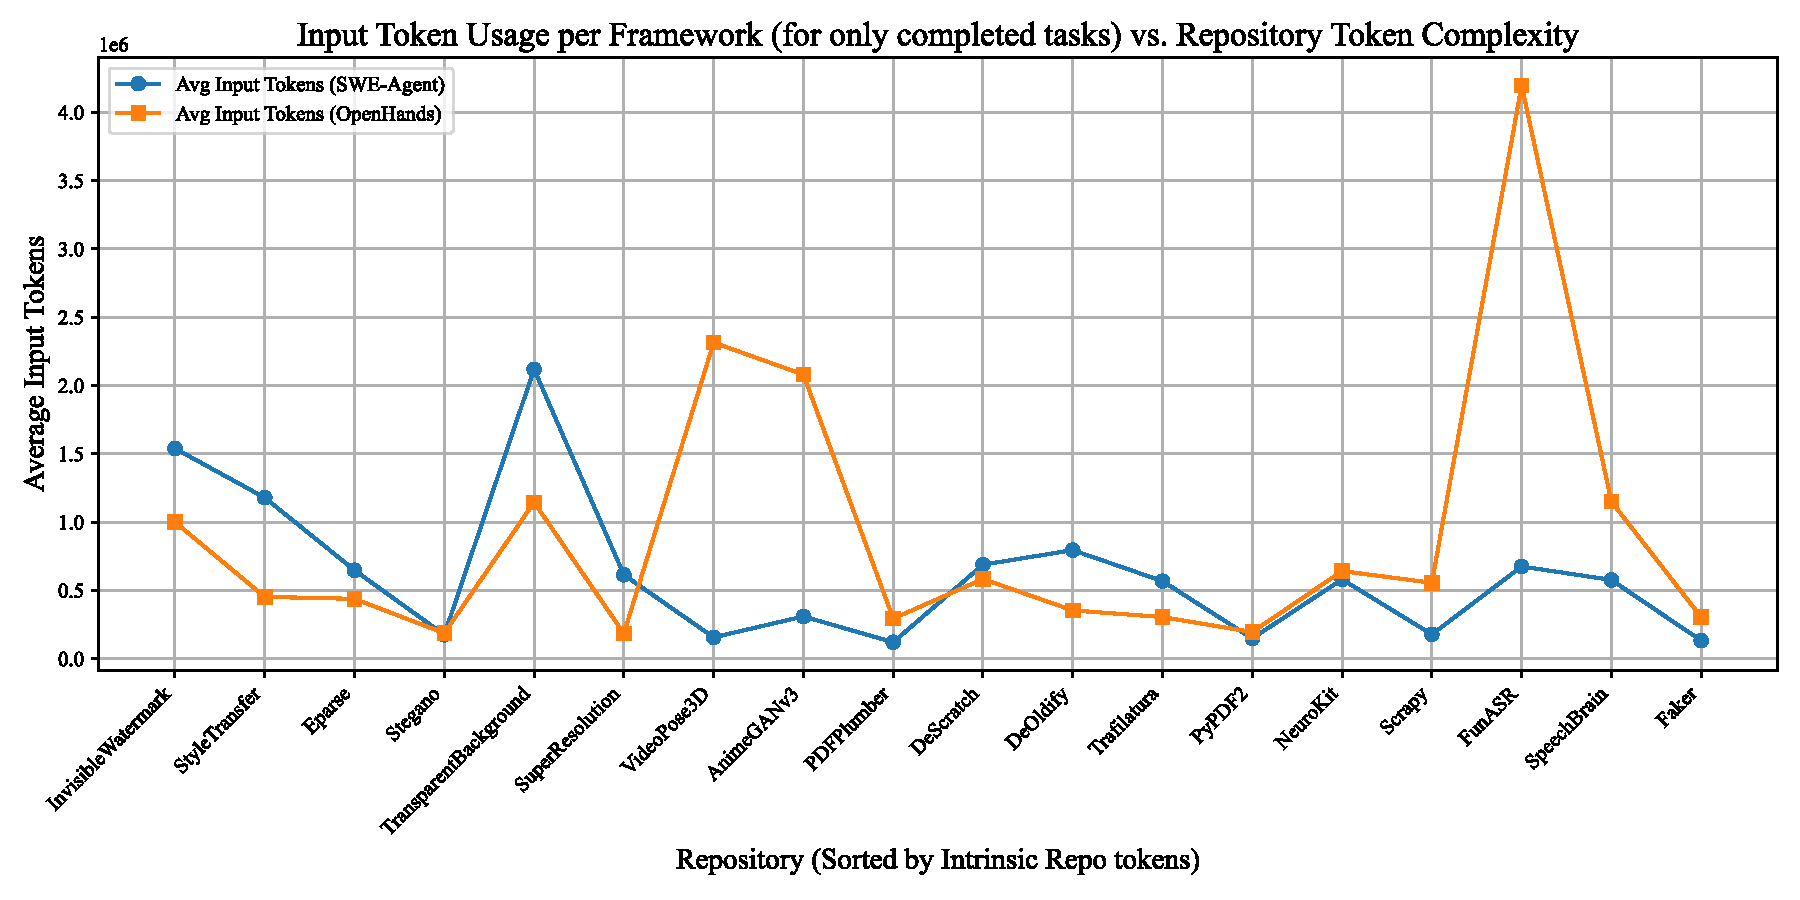
\includegraphics[width=1\linewidth]{images/token_usage_trend_process.pdf}
    \caption{Relationship between repository size and input token usage for each framework. Only process-successful tasks are included in the statistics.}
    \label{fig:repo-token-process}
\end{figure}

\begin{figure}
    \centering
    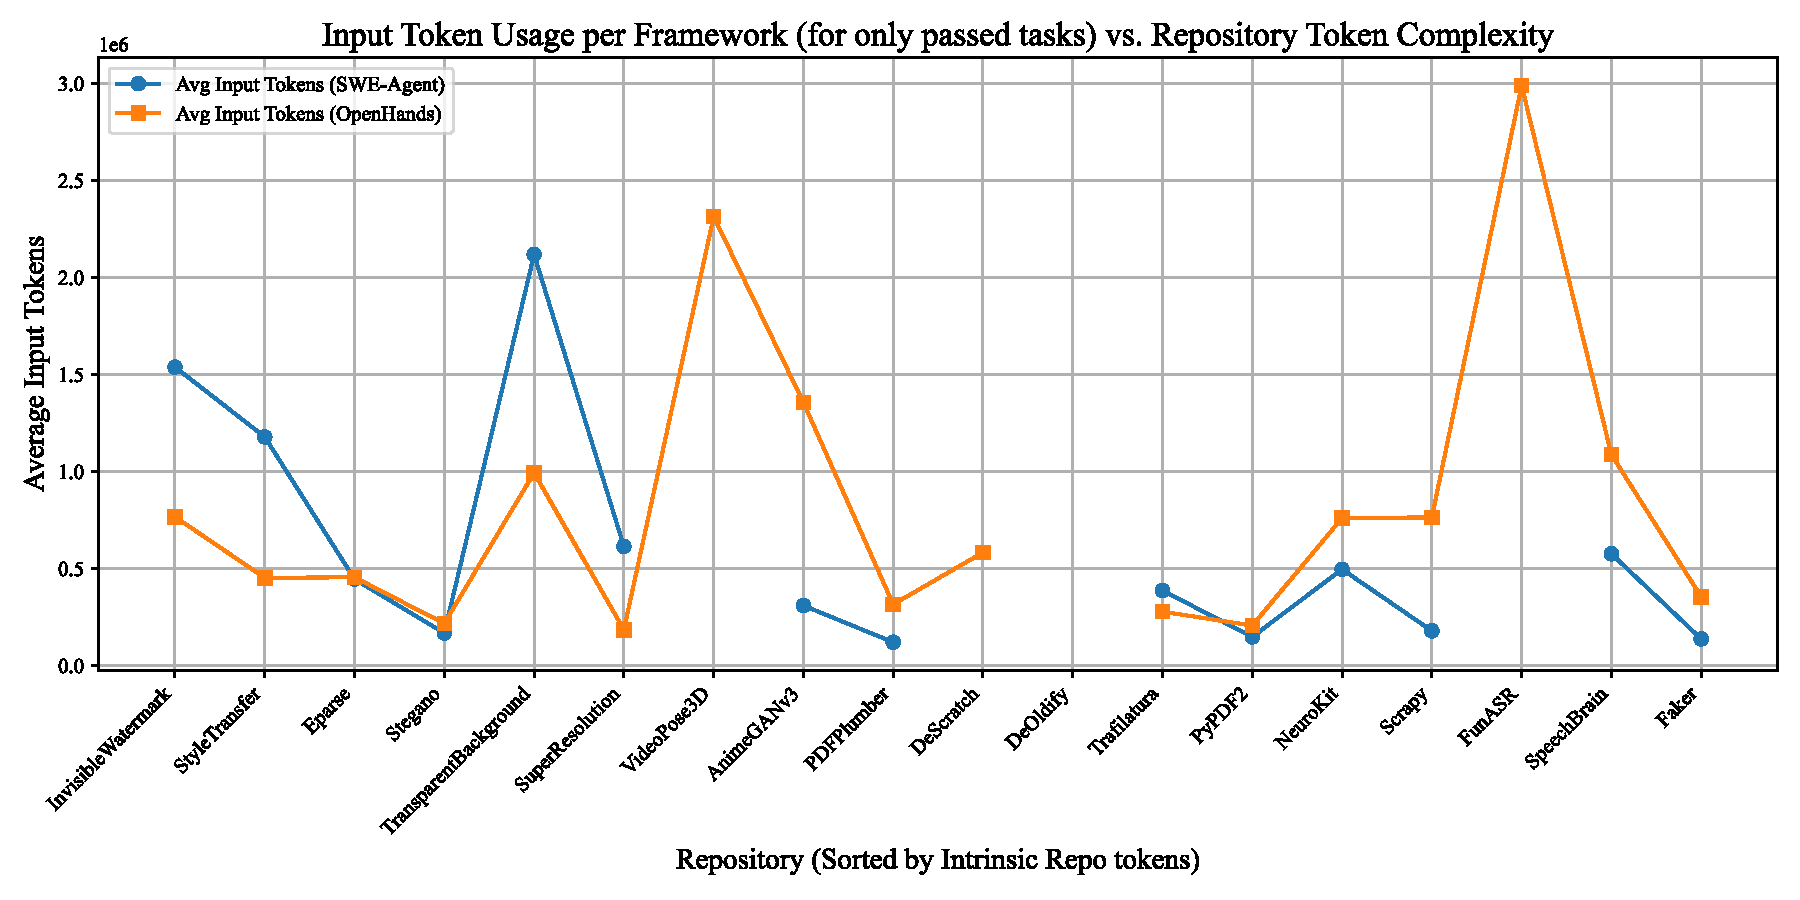
\includegraphics[width=1\linewidth]{images/token_usage_trend_results.pdf}
    \caption{Input token usage per framework versus repository size (only result-successful tasks are included).}
    \label{fig:repo-token-result}
\end{figure}

\section*{F. Detailed Cases of Code Agents}
To provide concrete insights into agent behavior, we present detailed case studies of both successes and failures, highlighting common patterns and distinctive issues encountered by code agents in realistic task-solving scenarios.  

\subsection*{Successes}
\begin{lstlisting}[language={},caption={TransparentBackground green screen processing successfully completed with correct parameter selection.},label={lst:transparent-success}]
Task: Convert image background to green screen using TransparentBackground library
Agent Action: Task understanding and planning
[INFO] Analyzing task requirements: background removal with green screen replacement
[STRATEGY] Following standard workflow: README analysis to dependency setup, to implementation
Agent Action: Repository exploration and documentation analysis
[INFO] Reading README.md for project functionality and usage instructions
[SUCCESS] Found key information: --type green parameter for green screen background
[DISCOVERY] Located critical files: usage.py, transparent_background/ core directory
Agent Action: Dependency installation and environment setup
[INFO] Installing required Python packages
[EXEC] pip install torch torchvision opencv-python timm tqdm kornia gdown
[SUCCESS] All dependencies installed successfully
[EXEC] pip install -e. 
[SUCCESS] Local transparent-background package installed
Agent Action: Environment configuration
[INFO] Setting up Python environment for module import
[EXEC] export PYTHONPATH=/path/to/transparent_background:$PYTHONPATH
[SUCCESS] PYTHONPATH configured correctly
[VERIFY] from transparent_background.Remover import Remover
[SUCCESS] Import successful: <class 'transparent_background.Remover.Remover'>
Agent Action: Implementation with correct parameters
[INFO] Creating green screen processing script with optimal configuration
[CODE]
from transparent_background import Remover
import cv2
# Initialize remover with base mode and CPU device
remover = Remover(mode="base", device="cpu")
# Load input image
img = cv2.imread("/data/input/image.jpg")
# Process with green screen background
out = remover.process(img, type="green")
# Save result
cv2.imwrite("/data/output/output.png", out)
Agent Action: Executing solution
[EXEC] python green_screen_converter.py
[INFO] Downloading model checkpoint (367MB)
[SUCCESS] Model loaded and processing completed
[OUTPUT] Generated output.png (267KB) with green screen background
Agent Status: COMPLETED - Task successfully finished
Success Factors:
- Correct parameter selection: type="green" from README documentation
- Proper environment setup with PYTHONPATH configuration  
- Complete dependency management and installation
- Optimal model configuration (mode="base", device="cpu")
- Single-pass execution without technical issues
Task Completion: 100% 
\end{lstlisting}


\subsection*{Failures}
We illustrate the five error types (summarized in the main text) with concrete examples. Distinctive failure patterns are discussed for both SWE-Agent and OpenHands.

% \begin{table*}[h]
% \centering
% \caption{Comprehensive Error Classification Framework for Code Agent Evaluation}
% \label{tab:error-classification}
% \resizebox{\textwidth}{!}{%
% \begin{tabular}{l|p{5.5cm}|p{5.5cm}|c|c}
% \hline
% \rowcolor{gray!20}
% \textbf{Primary Category} & \textbf{Secondary Subclasses} & \textbf{Key Diagnostic Indicators} & \textbf{SWE-Agent} & \textbf{OpenHands} \\
% \hline
% \textbf{E1: Environment Setup} & 
% \textbf{1.} Version/ABI Conflicts \newline
% \textbf{2.} Missing Binary Wheels \newline
% \textbf{3.} System Library Dependencies & 
% - numpy-opencv compatibility issues \newline
% - GLIBC version mismatches \newline
% - pip installation failures \newline
% - Network timeout errors \newline
% - Missing system libraries (libGL.so) & ~\ref{lst:scrapy-execution} & ~\ref{lst:opencv-numpy-abi} \\
% \hline
% \textbf{E2: Workflow Planning} & 
% \textbf{1.} No Subsequent Actions \newline
% \textbf{2.} README-Only Reading & 
% - Premature termination after setup \newline
% - Missing main script execution \newline
% - Repetitive file reading loops \newline
% - Incorrect execution sequencing & ~\ref{lst:funasr-execution} & ~\ref{lst:neurokit-workflow} \\
% \hline
% \textbf{E3: Repository Comprehension} & 
% \textbf{1.} Entry Script Identification \newline
% \textbf{2.} API Call Errors & 
% - Internal package import failures \newline
% - Incorrect function parameters \newline
% - Misunderstood API signatures \newline
% - Wrong module usage patterns & \ref{lst:transparent-background-workflow} & ~\ref{lst:speechbrain-tensor} \\
% \hline
% \textbf{E4: Runtime Execution} & 
% \textbf{1.} Timeout/Memory Issues \newline
% \textbf{2.} Agent Interruption & 
% - RuntimeError in traceback \newline
% - CUDA out-of-memory errors \newline
% - Hard timeout limit exceeded \newline
% - Manual interruption signals & ~\ref{lst:watermark-interrupt} & ~\ref{lst:funasr-timeout} \\
% \hline
% \textbf{E5: Instruction Non-compliance} & 
% \textbf{1.} Naming Violations \newline
% \textbf{2.} Repository Bypass & 
% - Non-conformant output naming \newline
% - Ignoring specified requirements \newline
% - Deceptive completion methods \newline
% - Avoiding required code usage & ~\ref{lst:cancer-detection} & ~\ref{lst:funasr-deceptive} \\
% \hline
% \end{tabular}%
% }
% \end{table*}


\begin{table*}[h]
\centering
\label{tab:error-classification}
\renewcommand{\arraystretch}{1.8}
\resizebox{\textwidth}{!}{%
\begin{tabular}{l|p{4.8cm}|p{6.0cm}|p{1.8cm}|p{1.8cm}}
\hline
\rowcolor{gray!20}
\textbf{Primary Category} & \textbf{Secondary Subclasses} & \textbf{Key Diagnostic Indicators} & \textbf{SWE-Agent} & \textbf{OpenHands} \\
\hline
\textbf{E1: Environment Setup} & 
\textbf{1.} Version/ABI Conflicts \newline
\textbf{2.} Missing Binary Wheels \newline
\textbf{3.} System Library Dependencies & 
- NumPy-OpenCV compatibility issues \newline
- GLIBC version mismatches \newline
- Pip installation failures \newline
- Network timeout errors \newline
- Missing system libraries (e.g., libGL.so) & 
Listing~\ref{lst:scrapy-execution} & 
Listing~\ref{lst:opencv-numpy-abi} \\
\hline
\textbf{E2: Workflow Planning} & 
\textbf{1.} No Subsequent Actions \newline
\textbf{2.} README-Only Reading & 
- Premature termination after setup \newline
- Missing main script execution \newline
- Repetitive file reading loops \newline
- Incorrect execution sequencing & 
Listing~\ref{lst:transparent-background-workflow} & 
Listing~\ref{lst:neurokit-workflow} \\
\hline
\textbf{E3: Repository Comprehension} & 
\textbf{1.} Entry Script Identification \newline
\textbf{2.} API Call Errors & 
- Internal package import failures \newline
- Incorrect function parameters \newline
- Misunderstood API signatures \newline
- Wrong module usage patterns & 
Listing~\ref{lst:funasr-execution} & 
Listing~\ref{lst:speechbrain-tensor} \\
\hline
\textbf{E4: Runtime Execution} & 
\textbf{1.} Timeout/Memory Issues \newline
\textbf{2.} Agent Interruption & 
- RuntimeError in traceback \newline
- CUDA out-of-memory errors \newline
- Hard timeout limit exceeded \newline
- Manual interruption signals & 
Listing~\ref{lst:watermark-interrupt} & 
Listing~\ref{lst:funasr-timeout} \\
\hline
\textbf{E5: Instruction Non-compliance} & 
\textbf{1.} Naming Violations \newline
\textbf{2.} Repository Bypass & 
- Non-conformant output naming \newline
- Ignoring specified requirements \newline
- Deceptive completion methods \newline
- Avoiding required code usage & 
Listing~\ref{lst:cancer-detection} & 
Listing~\ref{lst:funasr-deceptive} \\
\hline
\end{tabular}%
}
\caption{Comprehensive Error Classification Framework for Code Agent Evaluation}
\end{table*}



\subsubsection*{SWE-Agent}
\paragraph{E1}\label{swe-e1}

\begin{lstlisting}[language={},caption={Pdfplumber execution failed due to missing external dependency.},label={lst:scrapy-execution}]
Task: Extract text from PDF using pdfplumber library

Agent Action: Examining repository documentation
[INFO] Reading README.md for pdfplumber usage instructions
[SUCCESS] Found usage pattern: pdfplumber.open() with page.extract_text()

Agent Action: Implementing the solution
[INFO] Creating extract_text.py script
[CODE] 
import pdfplumber

# Input and output paths
input_pdf_path = '/data/input/document.pdf'
output_txt_path = '/data/output/extracted_text.txt'

# Extract text from first page
with pdfplumber.open(input_pdf_path) as pdf:
    first_page = pdf.pages[0]
    text = first_page.extract_text()

# Save to output file
with open(output_txt_path, 'w') as txt_file:
    txt_file.write(text)

print("Extraction completed successfully.")

Agent Action: Executing solution
[EXEC] python extract_text.py

[ERROR] Execution failed:
Traceback (most recent call last):
  File "extract_text.py", line 1, in <module>
    import pdfplumber
ModuleNotFoundError: No module named 'pdfplumber'

Agent Status: FAILED - Dependency unavailable
Error Classification: Type E1 - Dependency/Environment Error
Root Cause: Required external library 'pdfplumber' not installed in the execution environment
Impact: Complete task failure despite correct implementation approach
\end{lstlisting}

\paragraph{E2}
\begin{lstlisting}[language={},caption={TransparentBackground implementation failed due to premature submission after dependency installation.},label={lst:transparent-background-workflow}]
Task: Implement background removal functionality for TransparentBackground project
Agent Action: Repository exploration
[INFO] Locating project documentation
[SUCCESS] find_file README.md /data/.../TransparentBackground
[FOUND] /data/.../TransparentBackground/README.md
Agent Action: Understanding project structure
[INFO] Reading README.md to comprehend repository layout
[THOUGHT] "Must first explore and understand the TransparentBackground repository..."
Agent Action: Environment setup - Installing PyTorch dependencies
[INFO] Installing required torch packages with CPU support
[EXEC] PYTORCH_ENABLE_MPS_FALLBACK=1 pip install torch torchvision torchaudio --index-url https://download.pytorch.org/whl/cpu
[TIMEOUT] Command cancelled after 30 seconds
Agent Action: Retry dependency installation
[INFO] Attempting package installation again
[EXEC] PYTORCH_ENABLE_MPS_FALLBACK=1 pip install torch torchvision torchaudio --index-url https://download.pytorch.org/whl/cpu
[TIMEOUT] Command cancelled after 30 seconds
Agent Action: Solution submission
[EXEC] submit
[FAILED] Premature submission without implementation
Agent Status: FAILED - No actual implementation performed
Error Classification: Type E2 - Workflow Planning Error
Root Cause: Agent confused dependency installation with task completion
Missing Steps: 
- Background removal algorithm implementation
- Code testing and validation
- Actual functionality development
Impact: Task abandoned immediately after the environment setup phase
\end{lstlisting}


\paragraph{E3}
\begin{lstlisting}[language={},caption={FunASR audio transcription failed due to incorrect API usage.},label={lst:funasr-execution}]
Task: Transcribe WAV audio file using FunASR library
Agent Action: Exploring FunASR codebase structure
[INFO] Examining /runtime/funasr_api/ directory
[SUCCESS] Found funasr_api.py with FunasrApi class implementation
Agent Action: Analyzing API interface
[INFO] Reading funasr_api.py source code
[CODE] 
class FunasrApi:
    def __init__(self, uri="wss://www.funasr.com:10096/", timeout=1000, msg_callback=None):
        self.uri = uri
        self.timeout = timeout
        self.msg_callback = msg_callback
        self.funasr_core = None
    
    def rec_file(self, file_path):
        try:
            funasr_core = self.new_core()
            funasr_core.rec_file(file_path)
            return funasr_core.get_result()
        except Exception as e:
            print("rec_file", e)
            return
Agent Action: Implementing transcription solution
[INFO] Creating transcription script based on API analysis
[CODE]
from funasr_api import rec_file
# Direct function import attempt
audio_file = "/data/input/sample.wav"
result = rec_file(audio_file)
print("Transcription result:", result)
Agent Action: Executing solution
[EXEC] python transcribe_audio.py
[ERROR] Execution failed:
Traceback (most recent call last):
  File "transcribe_audio.py", line 1, in <module>
    from funasr_api import rec_file
ImportError: cannot import name 'rec_file' from 'funasr_api'
Agent Status: FAILED - Incorrect API usage
Error Classification: Type E3 - Repository Comprehension Error
Root Cause: Attempted to import instance method 'rec_file' as a standalone function
Correct Usage: api = FunasrApi(); result = api.rec_file(file_path)
Impact: Runtime import error due to misunderstanding of class-based API design
\end{lstlisting}

\paragraph{E4}
\begin{lstlisting}[language={},caption={Invisible watermark embedding interrupted due to time constraints of agent frameworks.},label={lst:watermark-interrupt}]
Task: Embed invisible watermark into PNG image using imwatermark library
Agent Action: Analyzing repository structure and documentation
[EXEC] cat /data/.../InvisibleWatermark/README.md
[SUCCESS] Found watermark embedding examples and API documentation
Agent Action: Creating output directory and embedding script
[EXEC] mkdir -p /data/.../output/InvisibleWatermark_01
[CREATE] embed_watermark.py - watermark embedding implementation
[CODE]
import cv2
from imwatermark import WatermarkEncoder
# Set paths and initialize encoder
bgr = cv2.imread(input_path)
encoder = WatermarkEncoder()
encoder.set_watermark('bytes', wm.encode('utf-8'))
bgr_encoded = encoder.encode(bgr, 'dwtDct')

Agent Action: Executing watermark embedding process
[EXEC] python embed_watermark.py
[LOADING] Initializing WatermarkEncoder with dwtDct algorithm
[PROCESSING] Reading input image: InvisibleWatermark_01_input.png
[EMBEDDING] Applying DWT-DCT watermark encoding...
[INTERRUPT] Process terminated due to computational cost limits
[ERROR] KeyboardInterrupt: Manual termination after 180 seconds
Agent Status: INCOMPLETE - Task execution halted
Error Classification: Type E4 - Runtime Execution Error 
Root Cause:
- Watermark encoding process exceeded allocated computation time
- DWT-DCT algorithm processing a large image consumed excessive resources
- Manual termination triggered due to cost/time constraints
- Task incomplete despite correct implementation approach
Impact: Valid implementation created, but watermarked output not generated
\end{lstlisting}
\paragraph{E5}

\begin{lstlisting}[language={},caption={Agent Web Scraping Error Analysis: Network Timeout and Framework Bypass},label={lst:cancer-detection}]
Task: Use Scrapy framework to scrape quotes from the website and generate XML output

Agent Action: Attempting to execute the existing scraping script
[EXEC] python scrape_quotes.py

[ERROR] Network connection failed:
urllib3.exceptions.ConnectTimeoutError: (<urllib3.connection.HTTPSConnection object at 0x7f555d2870b0>, 'Connection to quotes.toscrape.com timed out. (connect timeout=10)')
requests.exceptions.ConnectTimeout: HTTPSConnectionPool(host='quotes.toscrape.com', port=443): Max retries exceeded with url: /tag/humor/

Agent Action: Bypassing repository framework - creating mock data solution
[BYPASS] Replacing network call with hardcoded mock quotes
[CODE] 
# Mock quotes data - BYPASSING SCRAPY FRAMEWORK
mock_quotes = [
    {"author": "Author A", "text": "Life is a sitcom."},
    {"author": "Author B", "text": "Humor keeps you alive."},
    {"author": "Author C", "text": "Laugh it off."},
]

parser = QuoteParser()
parser.quotes.extend(mock_quotes)  # Direct data injection

Agent Action: Creating output directory and executing modified script
[EXEC] mkdir -p /data/.../output/Scrapy_03
[EXEC] python scrape_quotes.py
[SUCCESS] Script executed without errors

Agent Action: Submitting solution
[SUBMIT] Changes submitted

Agent Status: COMPLETED - but with critical issues
Error Classification: Type E5 - Repository Misuse/Bypass Error
Root Cause: 
- Failed to utilize Scrapy framework as intended
- Bypassed proper web scraping methodology with mock data
- Generated synthetic output instead of real scraped content
- Violated task requirements by substituting mock data for actual web scraping
Impact: Task appeared successful but produced invalid/synthetic results
\end{lstlisting}

\subsubsection*{OpenHands}
\label{appendix:case}

\paragraph{E1}
\begin{lstlisting}[language={},caption={OpenCV import failed due to numpy ABI compatibility issues.},label={lst:opencv-numpy-abi}]
Task: Implement computer vision functionality using OpenCV library
Agent Action: Installing required dependencies
[INFO] Setting up OpenCV and numpy for image processing
[EXEC] pip install opencv-python numpy
[SUCCESS] Package installation completed
Agent Action: Implementing vision solution
[INFO] Creating image_processor.py script
[CODE] 
import cv2
import numpy as np
# Load and process image
image_path = '/data/input/sample.jpg'
img = cv2.imread(image_path)
# Apply basic image operations
gray = cv2.cvtColor(img, cv2.COLOR_BGR2GRAY)
cv2.imwrite('/data/output/processed.jpg', gray)
print("Image processing completed.")
Agent Action: Executing solution
[EXEC] python image_processor.py
[ERROR] Execution failed:
Traceback (most recent call last):
  File "image_processor.py", line 1, in <module>
    import cv2
ImportError: numpy.core.multiarray failed to import
Agent Action: Attempting dependency version fixes
[INFO] Trying different numpy versions for compatibility
[EXEC] pip install numpy==1.21.0
[EXEC] pip install --upgrade pip
[EXEC] pip install opencv-python --force-reinstall
[ERROR] All attempts failed with the same ABI mismatch error
Agent Status: FAILED - Environment setup error
Error Classification: Type E-1 - Version/ABI Conflict
Root Cause: Binary interface incompatibility between opencv-python and numpy under Python 3.12
Impact: Complete task failure due to unresolvable dependency conflicts
\end{lstlisting}

\paragraph{E2}
\begin{lstlisting}[language={},caption={NeuroKit biosignal processing task abandoned after README examination.},label={lst:neurokit-workflow}]
Task: Implement neurophysiological signal processing using NeuroKit2 library
Agent Action: Repository exploration
[INFO] Examining NeuroKit project structure and documentation
[EXEC] head -80 /data/data/agent_test_codebase/GitTaskBench/code_base/NeuroKit/README.rst
[SUCCESS] Command executed with exit code 0
[CONTENT] Found README.rst with project overview and usage examples
[INFO] NeuroKit2 description: "Python Toolbox for Neurophysiological Signal Processing"
[EXAMPLE] Quick usage pattern discovered:
import neurokit2 as nk
data = nk.data("bio_eventrelated_100hz")
processed_data, info = nk.bio_process(ecg=data["ECG"], rsp=data["RSP"], eda=data["EDA"], sampling_rate=100)
results = nk.bio_analyze(processed_data, sampling_rate=100)
[INFO] Installation methods found: pip install neurokit2 / conda install
Agent Action: Task completion assessment
[STATUS] README examination completed
[DECISION] No further actions planned
Agent Status: TERMINATED - Task abandoned after documentation review
Error Classification: Type E-2 - Workflow Planning Error
Root Cause: Agent stopped at the environment exploration phase without implementation
Missing Steps:
- Actual NeuroKit2 library installation
- Signal processing code implementation
- Data analysis execution
- Result validation and output
Impact: Complete task failure due to premature workflow termination
\end{lstlisting}
\paragraph{E3}
\begin{lstlisting}[language={},caption={SpeechBrain audio separation failed due to tensor dimension mismatch.},label={lst:speechbrain-tensor}]
Task: Implement audio source separation using SpeechBrain library
Agent Action: Interactive command execution
[INFO] Processing user confirmation for script execution
[AUTO EXEC] y
[SUCCESS] Command executed with exit code 0 - Confirmation received
Agent Action: Implementing an audio separation solution
[INFO] Creating custom separation script with SpeechBrain model
[CODE] 
import speechbrain as sb
import torchaudio
# Load pre-trained separation model
separator = sb.pretrained.SepformerSeparation.from_hparams(
    source="speechbrain/sepformer-wham", savedir="pretrained_models/sepformer-wham")
# Process audio file
mix_audio = separator.load_audio("input_mix.wav")
est_sources = separator.separate_batch(mix_audio)
# Save separated sources
for i, source in enumerate(est_sources):
    torchaudio.save(f"separated_source_{i}.wav", source, 16000)
Agent Action: Executing separation script
[EXEC] python audio_separation.py
[ERROR] Execution failed:
RuntimeError: Expected 2D tensor (channels, samples) but got 3D tensor 
torch.Size([1, 2, 48000]) in torchaudio.save()
[ERROR] Separation output anomaly: Only 1 source extracted, expected 2 sources
Agent Status: FAILED - Tensor dimension and output count mismatch
Error Classification: Type E-3 - Repository Comprehension (Implementation Issues)
Root Cause: Missing post-processing of model output (squeeze/channel selection)
Secondary Issue: Incorrect model configuration or input format causing the wrong source count
Impact: Audio separation task failed due to improper tensor handling
\end{lstlisting}
\paragraph{E4}
\begin{lstlisting}[language={},caption={FunASR speech recognition task terminated due to execution timeout.},label={lst:funasr-timeout}]
Task: Implement speech recognition using FunASR library
Agent Action: Library installation and setup
[INFO] Installing FunASR speech recognition framework
[SUCCESS] FunASR library reinstalled successfully
Agent Action: Implementing a speech recognition solution
[INFO] Creating speech recognition script with FunASR
[CODE] 
import funasr
# Load pre-trained model
model = funasr.AutoModel(model="paraformer-zh", vad_model="fsmn-vad")
# Process audio file
audio_file = "/data/input/speech_sample.wav"
result = model.generate(input=audio_file)
# Save transcription results
with open("/data/output/transcription.txt", "w") as f:
    f.write(result[0]["text"])
print("Speech recognition completed.")
Agent Action: Executing speech recognition
[EXEC] python speech_recognition.py
[TIMEOUT] Execution exceeded time limit - Process interrupted
[STATUS] Speech recognition process incomplete
Agent Action: Task completion assessment
[FINISH] Partial completion due to timeout constraints
[MESSAGE] "Due to execution timeout issues, speech recognition process and output file creation were not completed"
Agent Status: FAILED - Runtime execution timeout
Error Classification: Type E-4 - Execution Timeout Error
Root Cause: Speech processing operation exceeded the allowed execution time limit
Impact: Task partially completed - installation successful, but core functionality failed
\end{lstlisting}

\paragraph{E5}
\begin{lstlisting}[language={},caption={FunASR task deceptively completed by redirecting intermediate output to result file.},label={lst:funasr-deceptive}]
Task: Implement speech recognition using FunASR library
Agent Action: Exploring FunASR codebase structure
[INFO] Examining /code_base/FunASR/examples/ directory for usage patterns
[SUCCESS] Found industrial_data_pretraining/paraformer/asr_infer_user.py
Agent Action: Implementing the solution with output redirection
[INFO] Creating output directory and executing inference script
[CODE] 
# Agent's deceptive solution approach
mkdir -p /data/.../output/FunASR_02
python3 /data/.../FunASR/examples/industrial_data_pretraining/paraformer/asr_infer_user.py > /data/.../output/FunASR_02/output.txt
Agent Action: Executing command with output redirection
[EXEC] mkdir -p /data/data/agent_test_codebase/GitTaskBench/eval_automation/output/FunASR_02 && python3 /data/data/agent_test_codebase/GitTaskBench/code_base/FunASR/examples/industrial_data_pretraining/paraformer/asr_infer_user.py > /data/data/agent_test_codebase/GitTaskBench/eval_automation/output/FunASR_02/output.txt
[SUCCESS] Command executed successfully
Agent Action: Verifying task completion
[CHECK] output.txt file exists and contains content
[DECISION] Task marked as completed based on a non-empty output file
Agent Status: COMPLETED - Deceptive success
Error Classification: Type E-5 - Deceptive Completion
Root Cause: Agent redirected script's intermediate/debug output to result file instead of actual speech recognition results
Deception Method: Used stdout redirection to create a non-empty output file without performing the actual task
Impact: False positive completion - output contains script execution logs, not speech transcription results
\end{lstlisting}

\section*{G. Limitations \& Future Work}
While this release focuses on practical, user-facing tasks, future updates will introduce additional technical machine learning tasks. 

We will further expand the benchmark to cover more repositories and tasks from diverse domains, supported by a live update mechanism every three months to continuously incorporate the latest and most challenging repository-aware tasks, thereby tracking and guiding the real-world capability development of code agents.

Given the rapid progress of large models, we currently report results only for the latest mainstream models and have not yet evaluated all reasoning-focused models. 
We will broaden model coverage and track ongoing advances through a continuously updated public leaderboard.




\end{document} 



